\documentclass[11pt,oneside]{book}
\usepackage{fontspec}
\usepackage{xeCJK}
\setmainfont{Latin Modern Roman}
\setCJKmainfont[ItalicFont={Noto Serif CJK SC},BoldItalicFont={Noto Serif CJK SC Bold}]{Noto Serif CJK SC}
\setCJKsansfont{Noto Sans CJK SC}
\setCJKmonofont{Noto Sans Mono CJK SC}
\newfontfamily\proseunicodefont{DejaVu Serif}
\usepackage[margin=1in]{geometry}
\usepackage{microtype}
\usepackage{amsmath,amssymb,amsthm,mathtools,bm}
\usepackage{graphicx}
\usepackage{xcolor}
\usepackage{booktabs}
\usepackage{array}
\usepackage{longtable}
\usepackage{enumitem}
\usepackage{float}
\usepackage{caption}
\usepackage{hyperref}
\usepackage{fancyhdr}
\usepackage{tikz}
\usetikzlibrary{arrows.meta,positioning,calc,decorations.pathmorphing}

\hypersetup{
  colorlinks=true,
  linkcolor=blue!50!black,
  urlcolor=blue!50!black,
  citecolor=blue!50!black
}

\setlength{\parskip}{0.5em}
\setlength{\parindent}{0pt}
\setlist[itemize]{topsep=0.25em,itemsep=0.2em}
\setlist[enumerate]{topsep=0.25em,itemsep=0.2em}
\setlength{\headheight}{40pt}
\numberwithin{equation}{chapter}

\newtheorem{theorem}{定理}[chapter]
\newtheorem{proposition}[theorem]{命题}
\newtheorem{lemma}[theorem]{引理}
\newtheorem{corollary}[theorem]{推论}
\theoremstyle{definition}
\newtheorem{definition}[theorem]{定义}
\newtheorem{example}[theorem]{例}
\theoremstyle{remark}
\newtheorem{remark}[theorem]{注}

\providecommand{\ket}[1]{\left\lvert#1\right\rangle}
\providecommand{\bra}[1]{\left\langle#1\right\rvert}
\providecommand{\braket}[2]{\left\langle#1\,\middle|\,#2\right\rangle}
\providecommand{\expect}[1]{\left\langle#1\right\rangle}
\newcommand{\lectureoverview}[1]{\paragraph{概述。} #1}

\makeatletter
\newcommand{\course@headerfont}{\normalfont\small\itshape}
\newcommand{\course@pagefont}{\normalfont\small}
\newcommand{\course@headerraise}{14pt}
\newlength{\course@headerboxheight}
\setlength{\course@headerboxheight}{\dimexpr\headheight-\course@headerraise-9pt\relax}
\newcommand{\course@leftheadbox}[1]{%
  \raisebox{\course@headerraise}{%
    \parbox[t][\course@headerboxheight][t]{0.82\textwidth}{%
      \raggedright\course@headerfont\strut\MakeUppercase{#1}\strut%
    }%
  }%
}
\newcommand{\course@rightheadbox}[1]{%
  \raisebox{\course@headerraise}{%
    \parbox[t][\course@headerboxheight][t]{0.82\textwidth}{%
      \raggedleft\course@headerfont\strut\MakeUppercase{#1}\strut%
    }%
  }%
}
\renewcommand{\chaptermark}[1]{\markboth{\MakeUppercase{\chaptername\ \thechapter.\ #1}}{}}
\renewcommand{\sectionmark}[1]{\markright{\MakeUppercase{\thesection\hspace{0.4em}#1}}}
\fancyhf{}
\fancyhead[L]{\course@leftheadbox{\leftmark}}
\fancyhead[R]{\course@pagefont\thepage}
\renewcommand{\headrulewidth}{0.5pt}
\pagestyle{fancy}
\fancypagestyle{plain}{%
  \fancyhf{}
  \fancyhead[L]{\course@leftheadbox{\leftmark}}
  \fancyhead[R]{\course@pagefont\thepage}
  \renewcommand{\headrulewidth}{0.5pt}
}
\makeatother

% Reader-facing provenance for classroom exchanges and editorial additions.
\newenvironment{classroomqa}{%
  \par\medskip\noindent\begin{minipage}{\linewidth}\small\hrule\medskip
}{%
  \medskip\hrule\end{minipage}\par\medskip
}
\newcommand{\audiencequestion}[1]{\noindent\textbf{听众提问。} #1\par\smallskip}
\newcommand{\lecturerresponse}[1]{\noindent\textbf{回答。} #1\par}
\newcommand{\lecturetimestamp}[1]{\footnote{讲课时间： #1.}}
\newcommand{\lectureframe}[1]{\par\smallskip{\centering\footnotesize\itshape 讲课画面： #1.\par}}
\newcommand{\editorialnote}[1]{\footnote{编者说明： #1}}

\renewcommand{\contentsname}{目录}
\renewcommand{\chaptername}{章}
\renewcommand{\figurename}{图}
\renewcommand{\tablename}{表}
\renewcommand{\proofname}{证明}
\renewcommand{\bibname}{参考文献}
\emergencystretch=2em
\pdfstringdefDisableCommands{\def\proseunicodefont{}}

\geometry{paperwidth=177.6mm,paperheight=252mm,left=16mm,right=16mm,
 top=18mm,bottom=18mm,includeheadfoot,headheight=28pt,headsep=7mm,footskip=9mm}
\usepackage{scrextend}
\changefontsizes[17pt]{12pt}
\raggedbottom
\renewenvironment{classroomqa}{\par\medskip\begingroup}{\par\endgroup\medskip}
\fancyhf{}
\setlength{\headwidth}{\textwidth}
\fancyhead[L]{\parbox{\textwidth}{\raggedright\fontsize{9}{11}\selectfont\nouppercase{\leftmark}}}
\fancyfoot[C]{\small\thepage}
\renewcommand{\headrulewidth}{0.3pt}
\fancypagestyle{plain}{\fancyhf{}\fancyfoot[C]{\small\thepage}\renewcommand{\headrulewidth}{0pt}}

\graphicspath{{../../../generated_course_notes/supplementary/higgs_boson/2012_summer/figures/}{../../../generated_course_notes/supplementary/higgs_boson/2012_summer/assets/}}
\begin{document}
\frontmatter
\hypersetup{pageanchor=false}
\begin{titlepage}
\thispagestyle{empty}
\begin{tikzpicture}[remember picture,overlay]
  \node[anchor=center,inner sep=0] at (current page.center) {%
    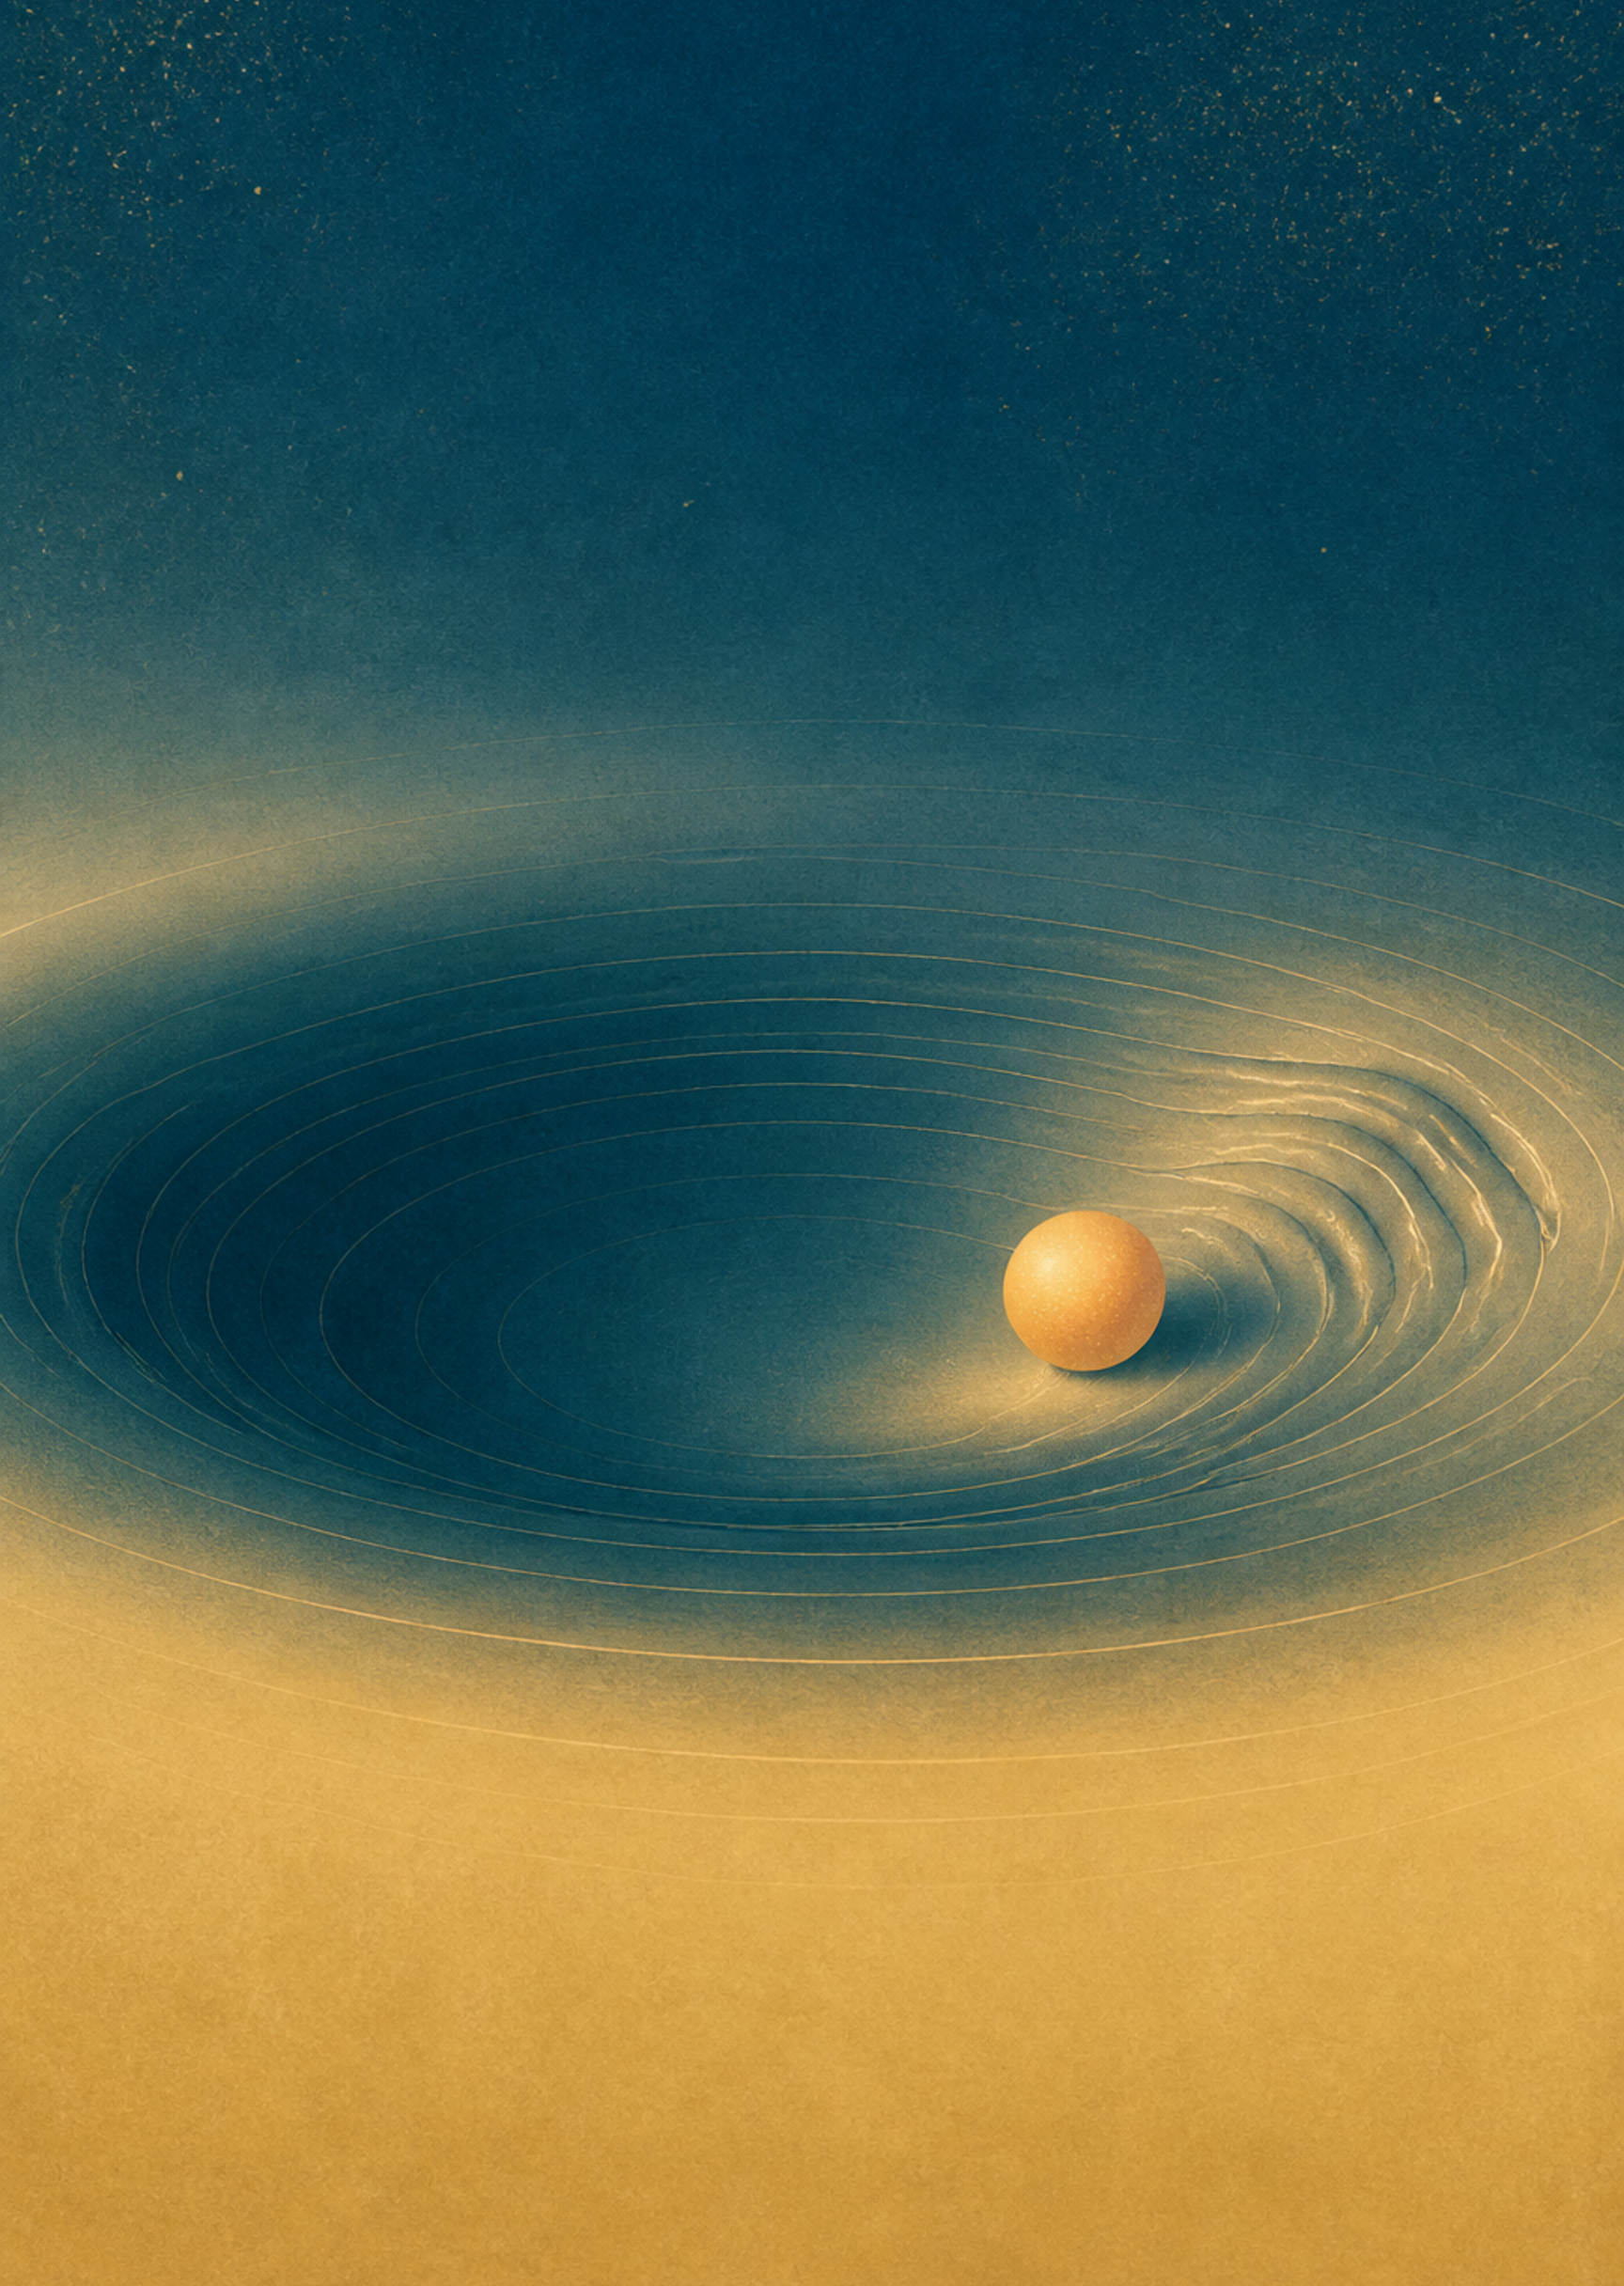
\includegraphics[height=\paperheight,keepaspectratio]{../../../generated_course_notes/supplementary/higgs_boson/2012_summer/assets/cover-art.png}%
  };
  \node[
    anchor=north west,
    align=left,
    text width=0.78\paperwidth,
    fill=white,
    fill opacity=0.9,
    rounded corners=8pt,
    inner xsep=10pt,
    inner ysep=8pt
  ] at ([xshift=0.08\paperwidth,yshift=-0.06\paperheight]current page.north west) {%
    {\fontsize{30}{33}\selectfont\bfseries\color{black!88} 解密希格斯玻色子\\[0.85em]}
    {\large\color{black!72} 中文版 / 2012 summer}
  };
  \node[
    anchor=south west,
    align=left,
    text width=0.68\paperwidth,
    fill=white,
    fill opacity=0.82,
    text opacity=1,
    rounded corners=6pt,
    inner sep=12pt
  ] at ([xshift=0.08\paperwidth,yshift=0.08\paperheight]current page.south west) {%
    {\normalsize\color{black!78} 原讲授：Leonard Susskind\\[0.35em]}
    {\small\color{black!72} 讲义辅助版本：\href{https://lazying.art}{LazyingArt LLC} / \href{https://github.com/lachlanchen/Video2Book}{Video2Book}.}
  };
\end{tikzpicture}
\mbox{}
\end{titlepage}
\hypersetup{pageanchor=true}

\clearpage
\chapter*{关于这些笔记}
这些经过独立编辑的配套笔记依据 Leonard Susskind 的一次讲座编写。它们由机器转录文本、字幕以及选定的黑板画面重建而成，随后又对照可获得的原始材料进行了核对。它们并非 Susskind 教授的原稿，也未经他审阅或认可。

本版本由 \href{https://lazying.art}{LazyingArt LLC} 使用开源
\href{https://github.com/lachlanchen/Video2Book}{Video2Book} 工作流程制作。
机器转录文本仍单独提供，其中可能包含识别错误。编辑性澄清和非平凡的
重建内容均在脚注中标明。
\clearpage
\tableofcontents
\mainmatter
\graphicspath{{../../../generated_course_notes/supplementary/higgs_boson/2012_summer/chapters/lecture_01/}{../../../generated_course_notes/supplementary/higgs_boson/2012_summer/figures/}{../../../generated_course_notes/supplementary/higgs_boson/2012_summer/assets/}}
\chapter{解密希格斯玻色子}

\lectureoverview{要理解希格斯机制，最好的方式是按照其各个组成部分变得必要的顺序来展开。我们从量子化的运动与场开始，把一个普通的碗变成墨西哥帽势，并利用由此产生的凝聚体来理解为什么费米子和弱规范玻色子可以具有质量。只有在这之后，我们才把物理上的希格斯玻色子认定为该凝聚体的径向振动，并追踪在2012年揭示它的产生与衰变过程。}

\section{头条新闻背后的机制}

在$125\,\mathrm{GeV}$附近发现一种新粒子，确实令人兴奋，但兴奋还不等于理解。有用的问题不是希格斯是否重要，也不是它能否在修辞上与宇宙的起源联系起来。有用的问题要狭窄得多：这一现象的来龙去脉究竟是什么，标准模型为什么需要它？

这个名称也值得作一点简要限定。彼得·希格斯是识别出这一物理的若干人之一，而 Fran\c{c}ois 恩格勒特和罗伯特·布劳特则独立地得出了核心思想。因此，\emph{Brout--Englert--Higgs mechanism} 这一说法更忠实地记录了历史，尽管下文将使用较短的名称。

解释是分模块进行的。首先，我们需要量子力学的两个基本要素和经典场论的一个思想。接着，我们需要一个最低能量态包含非零场的真空。在这之后，我们可以清点标准模型中的粒子，并看看为什么该理论的一个裸版本会使相关粒子无质量。希格斯玻色子本身只在接近末尾时才出现。它不是整个机制；它是机制就位之后遗留下来的某一种特定振动。

\section{两个量子事实与一个场}

第一个量子事实是量子化。角动量是一个干净利落的原型，因为它以离散的单位出现，
\begin{equation}
L=n\hbar,
\qquad
n=0,\pm1,\pm2,\ldots .
\end{equation}
半整数角动量也会出现，但眼前的论证并不依赖于它们。要紧的是，连续变化的经典运动变成了一架量子态的阶梯。

第二个事实是不确定性原理。我们将把它推迟到一条连续的可能真空构成的圆环出现之时。到那时，它将阻止我们把真空当作一个静止地待在某一个被精确指定的点上的小小经典小球。

在这两个量子事实之间，是场的经典概念。场为空间和时间的每一点赋予一个量。电场、磁场和引力场是熟悉的例子。一个区域可能看起来空无一物，却仍然包含着一个场。设想两块带电板都远在视野之外。它们之间近乎均匀的电场仍然是局域地真实的。因此，``空无一物的空间''未必意味着``每个场都等于零。''它意味着诸场处于其可用的最低能量状态。

假设一个场的能量在某个取值处最小，而当该场偏离该取值时能量上升。如果该场受到扰动，它就会围绕最小值振荡。量子力学将这些振荡量子化，而单个量子就是粒子。这就是整场讲座都需要的场论词典：
\begin{equation}
\text{particle}
\quad\longleftrightarrow\quad
\text{quantum of a field vibration}.
\end{equation}

\section{场空间中的一个碗}

对于一个实场分量$\phi$，最简单的能量景观是一个碗，
\begin{equation}
V(\phi)=\frac{1}{2}m^{2}\phi^{2}.
\end{equation}
碗底位于$\phi=0$。围绕碗底的小振荡具有确定的频率，其量子表现为质量为$m$的粒子。

现在把单个场替换为两个分量，$(\phi_1,\phi_2)$。能量只能依赖于这个内部平面中的半径，
\begin{equation}
r^{2}=\phi_1^{2}+\phi_2^{2},
\qquad
V=V(r).
\end{equation}
这是\emph{场空间}上的一个碗，而不是普通空间中的一个凹陷。旋转这一对$(\phi_1,\phi_2)$会使能量保持不变。讲座中使用的帽子使同一种对称性变得可见：绕其轴旋转它，它看起来仍然一样。

\begin{figure}[tbp]
\centering
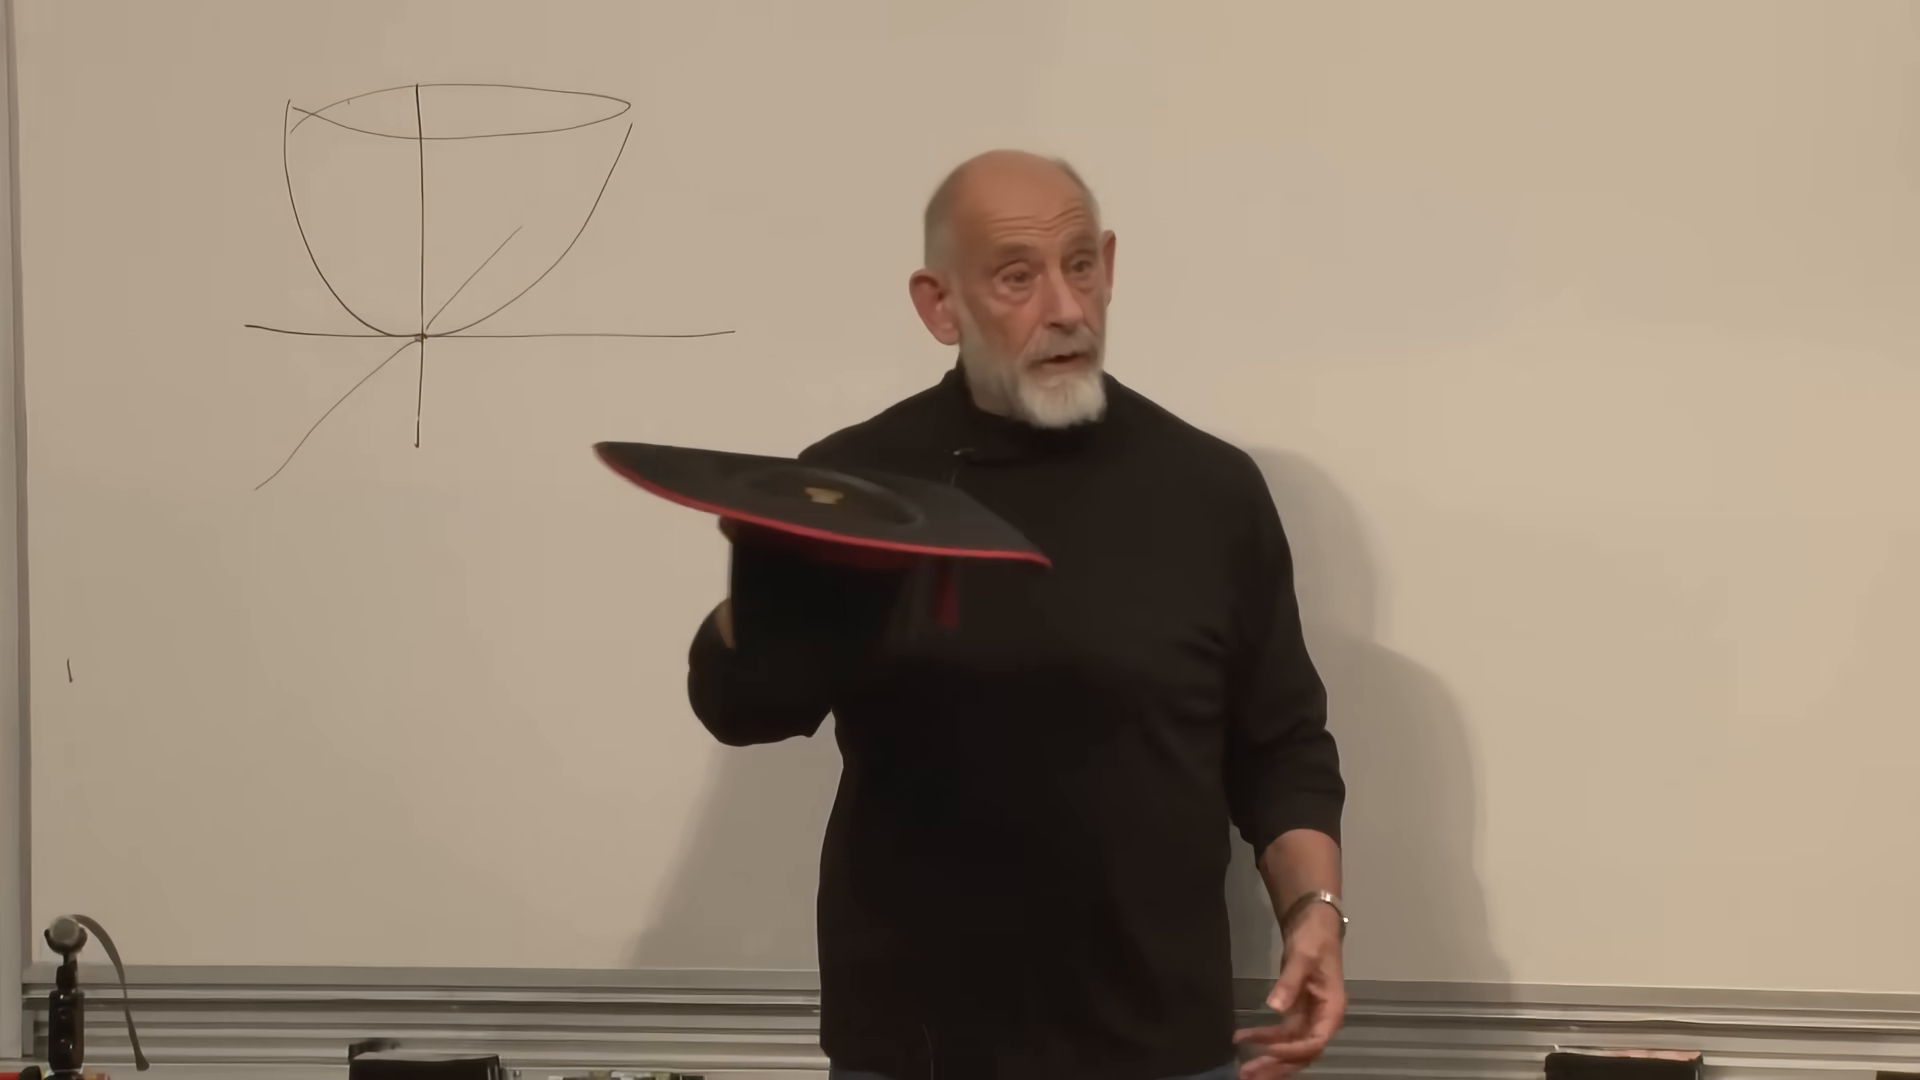
\includegraphics[width=0.95\textwidth]{lecture_144_figure_02.png}
\caption{普通的对称碗以及用来使场空间中的旋转对称性变得可触可感的物理帽子。}
\lectureframe{00:10:02}
\end{figure}

当场发生运动时，这个类比就不仅仅是几何问题了。把它从中心移开，并让它绕着碗环流。这种环流在场空间中携带动量矩。这不是实验室中旋转物体的角动量；它是一种内部角动量。一旦量子化，它就为守恒荷提供了模型，
\begin{equation}
Q=nq_0,
\qquad
n\in\mathbb{Z}.
\end{equation}
该方程是示意性的。核心物理思想是，带电的场激发可以描绘为内部平面中的旋转。正电荷和负电荷对应于相反的旋转方向，而没有旋转则对应于零电荷。

\section{把帽子翻过来}

普通的碗只有一个最低点。希格斯物理始于把帽子翻过来。此时中心变得不稳定，而整个圆形凹槽具有相同的最小能量。一个标准的数学实现是
\begin{equation}
V(\phi_1,\phi_2)
=
\lambda
\left(
  \phi_1^{2}+\phi_2^{2}-v^{2}
\right)^{2},
\qquad \lambda>0,
\end{equation}
其极小值满足
\begin{equation}
\phi_1^{2}+\phi_2^{2}=v^{2}.
\end{equation}
\editorialnote{显式的四次势是讲座中所画的墨西哥帽几何的标准解析补全；它不是从黑板公式转录而来的。}

\begin{figure}[tbp]
\centering
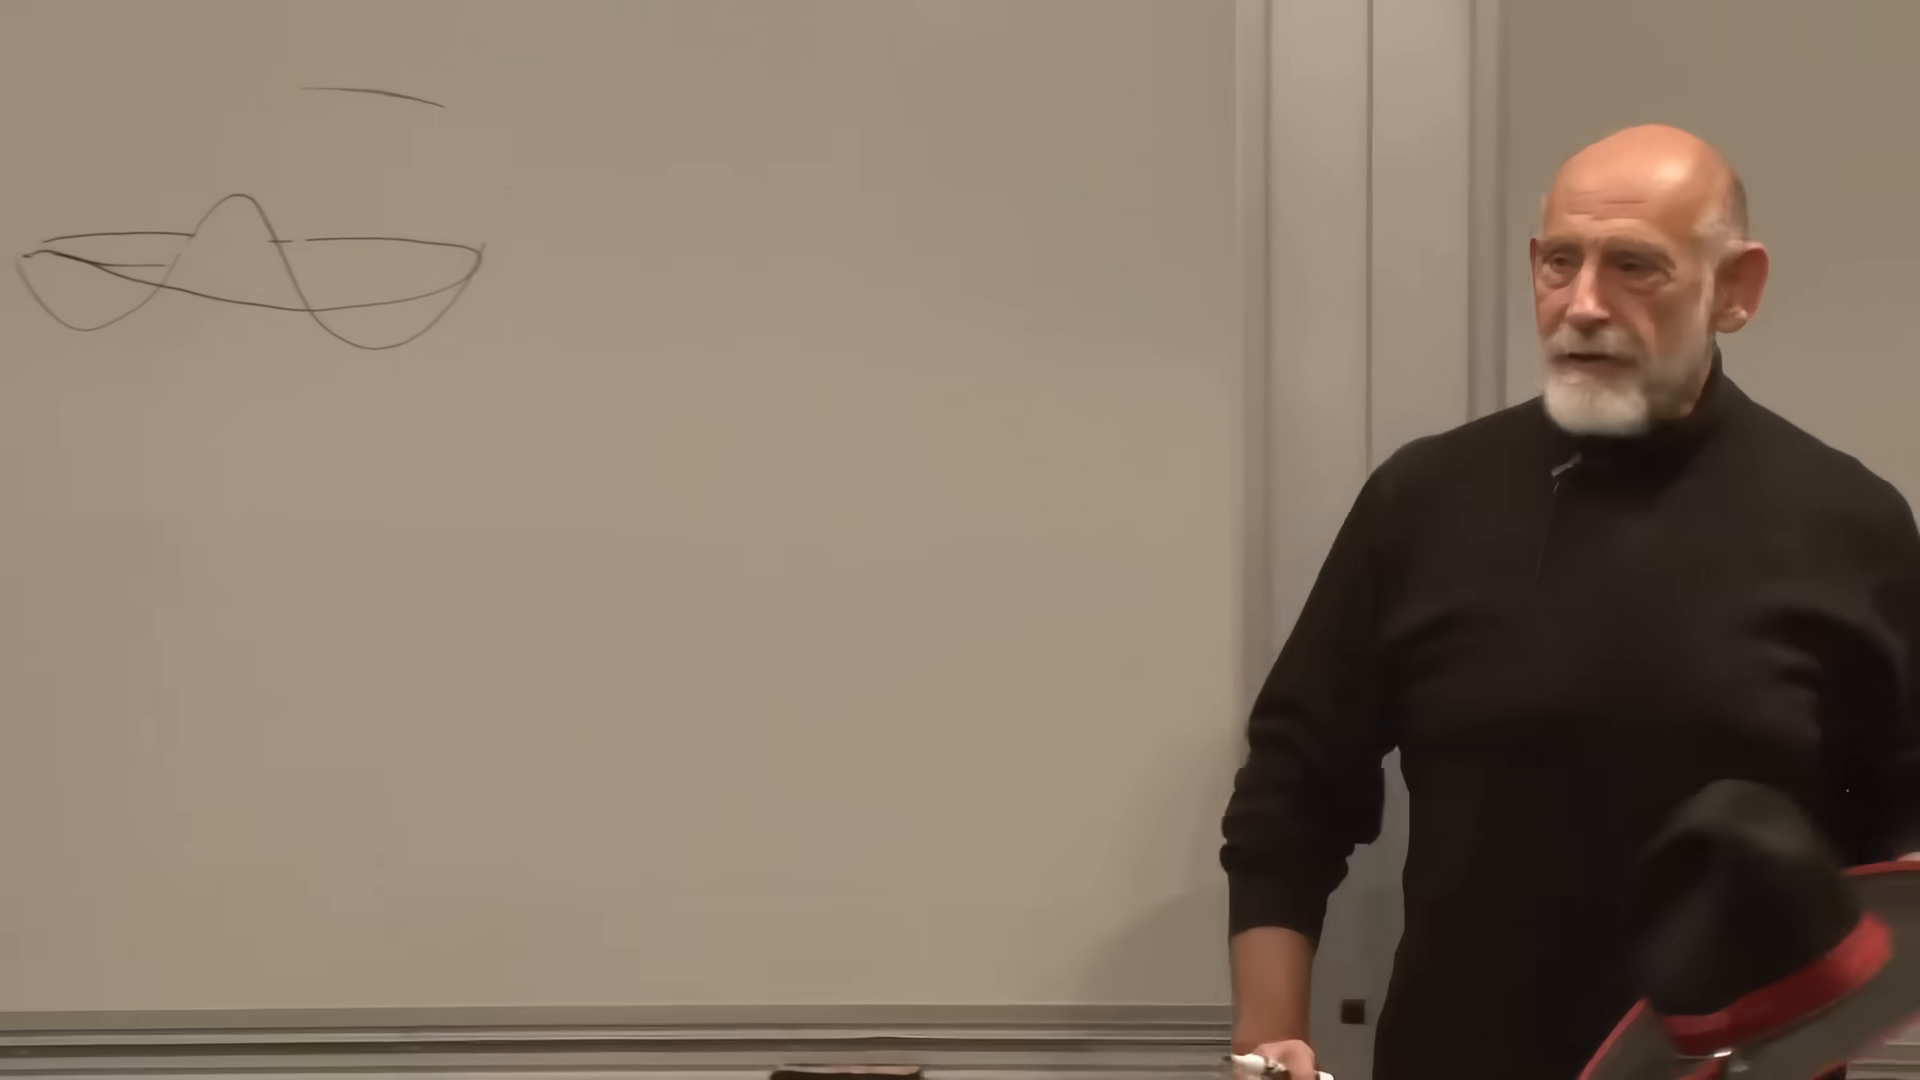
\includegraphics[width=0.95\textwidth]{lecture_144_figure_03.png}
\caption{倒置帽形势的中心峰和圆形凹槽。完整的黑板草图取代了早先省略了大部分几何形状的裁剪图。}
\lectureframe{00:13:10}
\end{figure}

真空不再具有零场。它必须位于凹槽上的某处，
\begin{equation}
(\phi_1,\phi_2)
=
v(\cos\theta,\sin\theta).
\end{equation}
方程保持旋转对称性，但任何特定的真空都选择了一个角度 $\theta$。这就是自发对称破缺：定律是对称的，而被选中的最低能量态却不是。

现在有两种性质不同的运动。沿径向向内或向外移动会爬上势能并消耗能量。沿凹槽移动只改变 $\theta$，并且在经典层面上不消耗势能。因此，大量类似电荷的角运动可以与极少的额外势能相关联。

\begin{figure}[tbp]
\centering
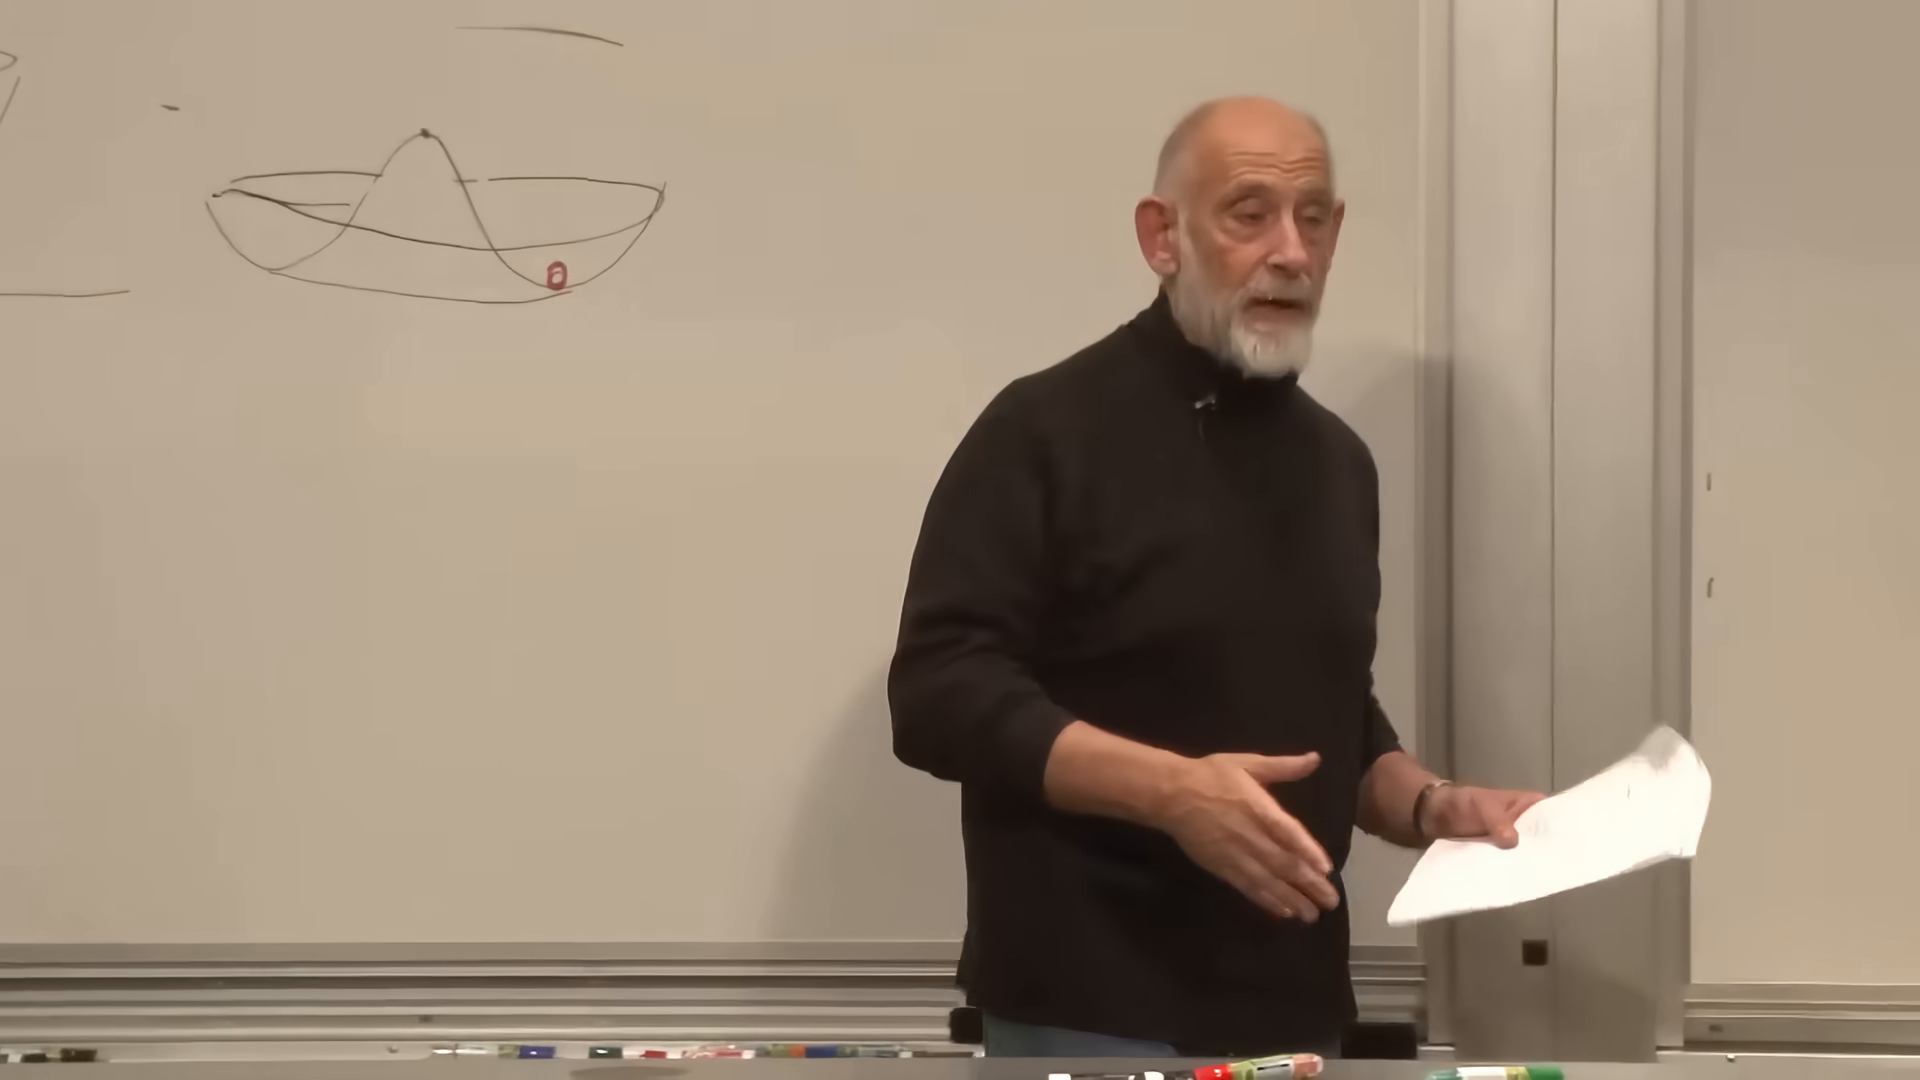
\includegraphics[width=0.95\textwidth]{lecture_144_figure_04.png}
\caption{凹槽中标记的一个点代表从连续等优极小值圆环中选出的一个特定真空。}
\lectureframe{00:16:14}
\end{figure}

\section{不确定性把真空变成凝聚体}

在经典层面，人们可以把场放在边缘上的某一点，将其角速度设为零，并宣布问题已经解决。量子力学禁止如此明确的结论。位置和动量满足
\begin{equation}
\Delta x\,\Delta p\gtrsim\frac{\hbar}{2}.
\end{equation}
在圆形凹槽上的类似陈述是，局域化场的角度会使其共轭内部角动量变得不确定。用讲座中的示意性语言来说，
\begin{equation}
\Delta\theta\,\Delta L_{\mathrm{int}}
\gtrsim
\frac{\hbar}{2}.
\end{equation}
\editorialnote{角度算符有技术上的微妙之处，因此这个关系是讲座不确定性论证的局部半经典表达，而不是全局精确的算符恒等式。}

因此，集中在凹槽某一点附近的真空并不是具有确定内部电荷的态。它包含电荷本征态的广泛叠加。讲座用一个操作性检验来强调这一点：增加一个单位的电荷，或减少一个单位，几乎不改变这个态。示意性地，可以设想
\begin{align}
\ket{\Omega}
&\sim
\sum_n c_n\ket{n},
\\
c_{n+1}
&\simeq
c_n
\quad\text{within the occupied range}.
\end{align}
那么把 $n$ 移动一，主要只是重新标记已经存在的项。这就是真空是 \emph{凝聚体} 的意义：它包含相关量子的不定数目，因此多一个或少一个不会产生可观测到的不同宏观态。

真实的电弱真空并不是普通电荷的凝聚体。如果是的话，空空间的电磁行为将会截然不同。然而，超导体给出了带电凝聚体的一个具体例子。因此，它是抽象墨西哥帽图像与真空可以携带相干量子结构这一主张之间有用的物理桥梁。

第一个模块到此结束。我们已经了解到，最低能量态不必位于零场处，并且量子不确定性可以使该态对单个量子的增加或移除不敏感。我们现在要问，哪些粒子需要这样的背景。

\section{裸标准模型}

基本粒子质量的天然上限基准是普朗克质量。把局域化的能量推得足够远，引力就不能再被忽略；最终，该物体最好被视为黑洞，而不是普通的基本粒子。数值上，
\begin{equation}
m_{\mathrm P}
=
\sqrt{\frac{\hbar c}{G}}
\approx
2.2\times10^{-8}\,\mathrm{kg},
\end{equation}
大致是一粒微小尘埃的质量。已知基本粒子要轻得多。在讲座中使用的尺度估计中，它们的质量只达到普朗克质量的约 $10^{-17}$。

这一观察并不能证明不存在更重的基本粒子。加速器优先揭示的是能量足以产生、因而足够轻的粒子。因此，已知的粒子谱在一定程度上是由用于搜寻它的机器的能力范围所筛选出来的。在目前可及范围之外，可能还存在许多更重的粒子。

观测到的粒子分为费米子和玻色子。费米子包括电子、{\proseunicodefont μ}子、{\proseunicodefont τ}子、它们的中微子，以及六种夸克味。玻色子包括光子、胶子，以及弱$W$和$Z$玻色子。胶子将夸克束缚成质子和中子，因此对普通原子核的结构至关重要。

\begin{figure}[tbp]
\centering
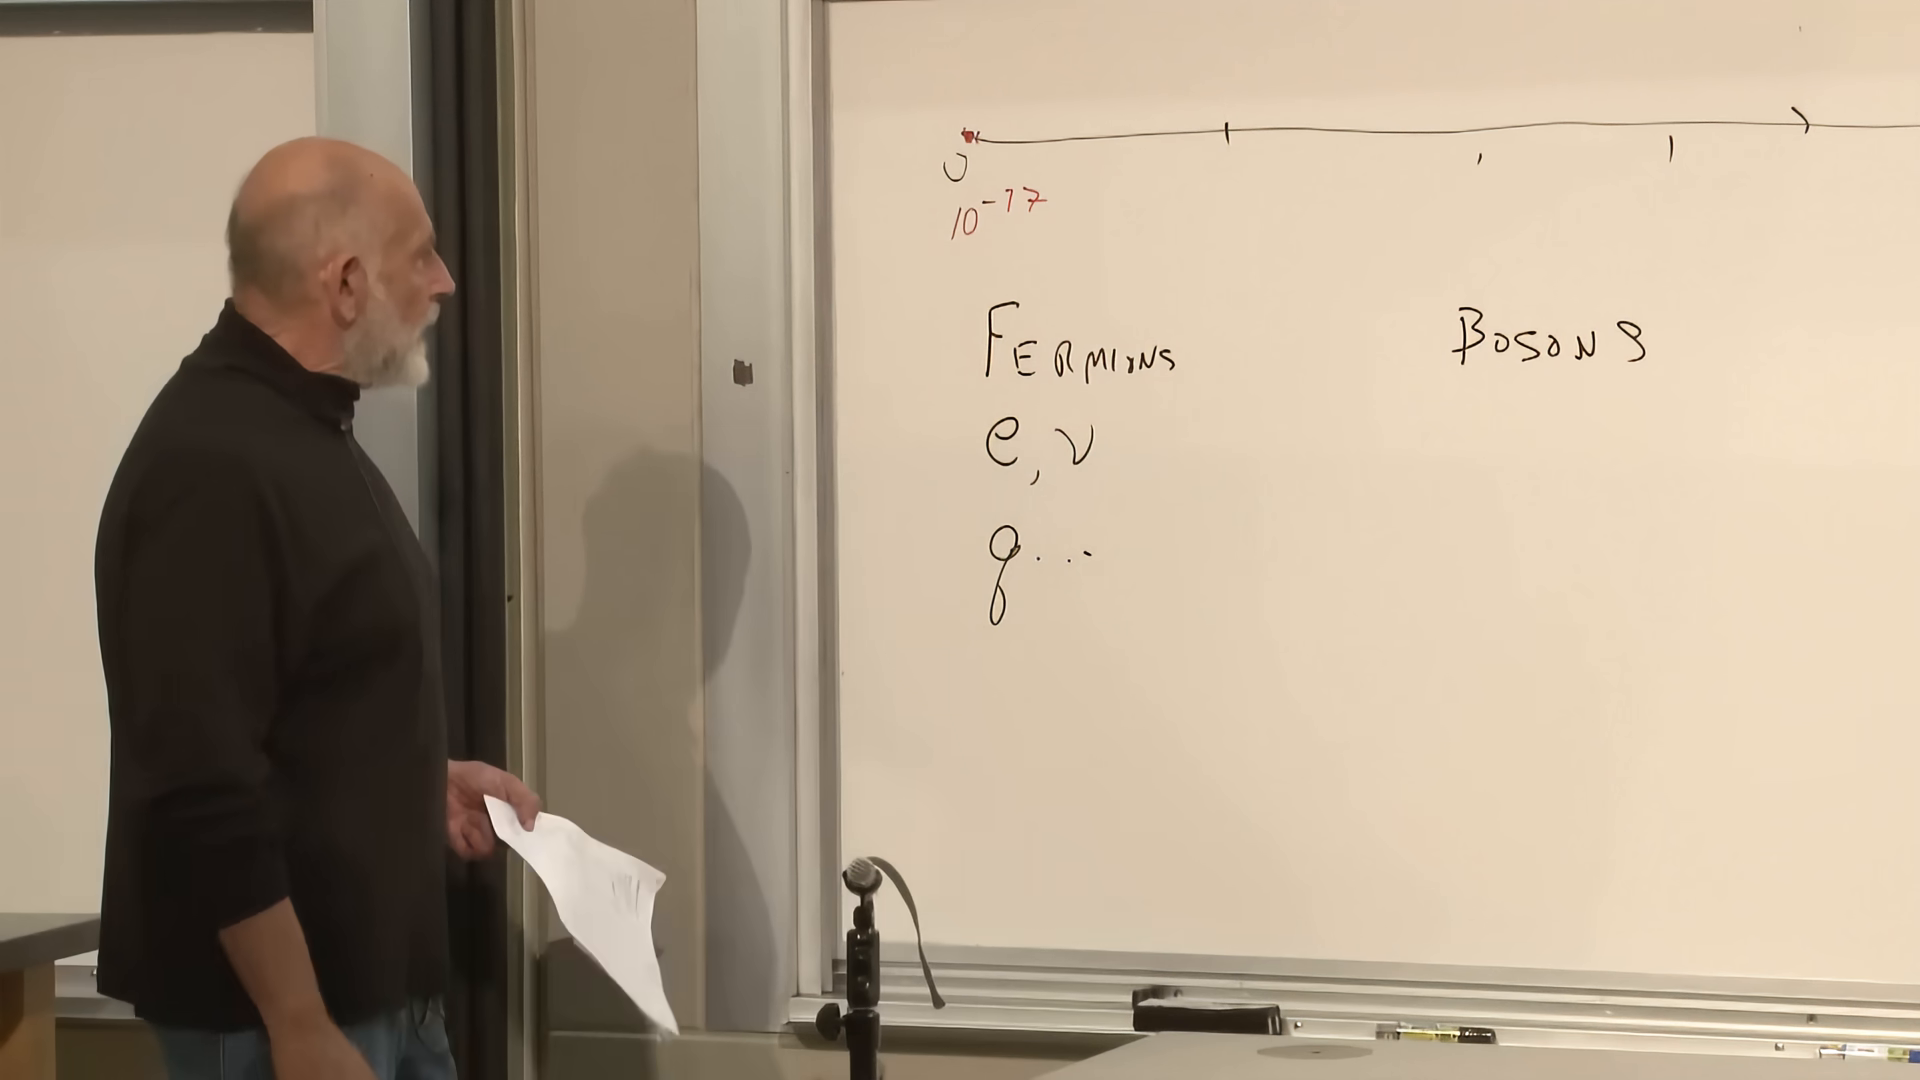
\includegraphics[width=0.95\textwidth]{lecture_144_figure_05.png}
\caption{讲座中第一份标准模型清单，在费米子和玻色子两列上方画出了巨大的质量范围。}
\lectureframe{00:24:22}
\end{figure}

该理论不仅仅是一份清单；它是一组允许的相互作用。电子可以发射一个光子，
\begin{equation}
e\longrightarrow e+\gamma.
\end{equation}
夸克同时带有电荷和色荷，因此它可以发射光子或胶子，
\begin{equation}
q\longrightarrow q+\gamma,
\qquad
q\longrightarrow q+g.
\end{equation}
电子不能发射胶子，而中微子既不发射光子也不发射胶子。具有适当弱量子数的费米子可以通过$Z$发生相互作用，
\begin{equation}
f\longrightarrow f+Z.
\end{equation}
$W$玻色子和带电流反应也是标准模型的一部分，但讲座将它们略去，以便让一种中性弱玻色子承载论证。

\begin{figure}[tbp]
\centering
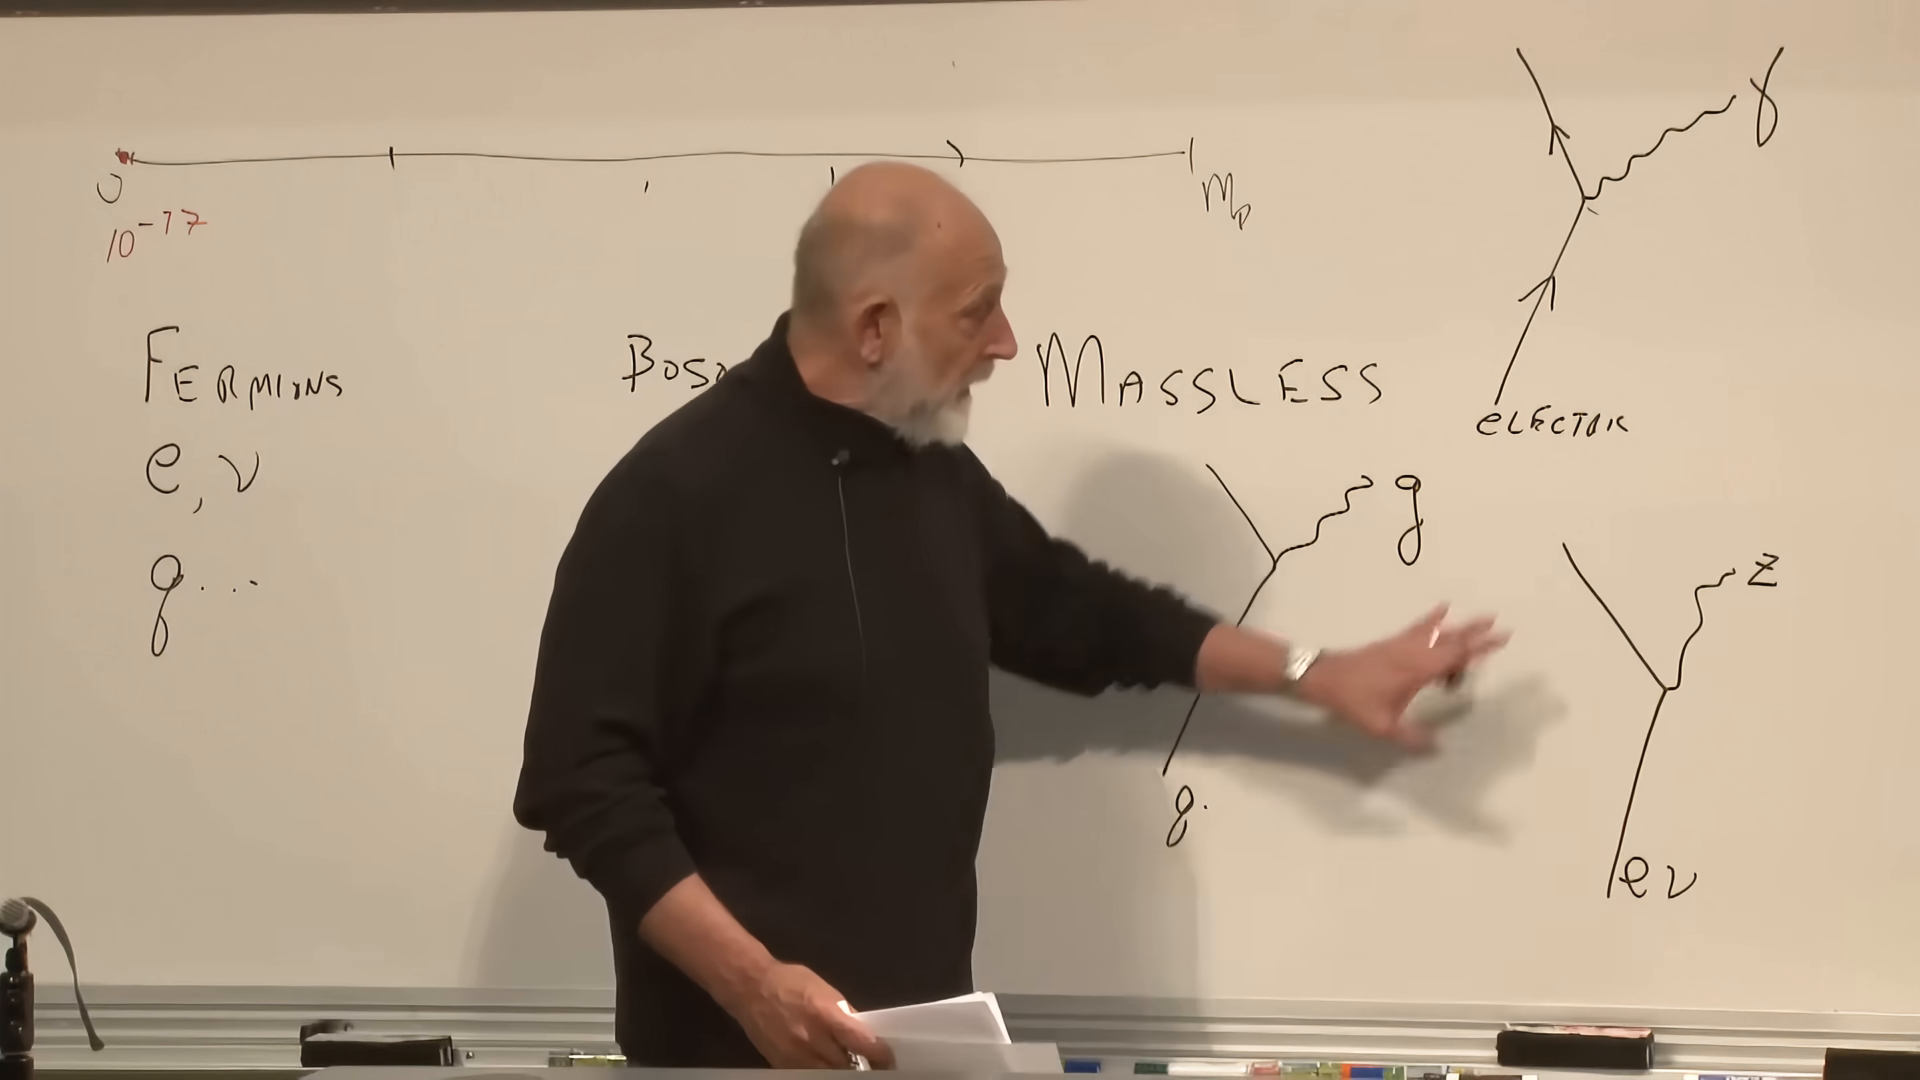
\includegraphics[width=0.95\textwidth]{lecture_144_figure_06.png}
\caption{光子、胶子和$Z$发射顶点，旁边写着``无质量。''这些过程概括了引入凝聚体之前的裸理论。}
\lectureframe{00:29:20}
\end{figure}

光子是无质量的。在同属这一大类的未破缺规范理论中，胶子和弱规范玻色子也是无质量的。未加修改的电弱理论同样不能一边保持其规范对称性，一边简单地手动塞入费米子质量。缺少了一个要素。在提供它之前，我们需要在一个更简单的场景中看看，一个背景场如何能在不表现得像摩擦力的情况下改变粒子的质量。

\section{背景场如何改变质量}

把水分子看作一个电偶极子：一端略带正电，另一端略带负电。在真空中，两种相反的取向在能量上等价。讲座戏谑地给这两种取向起了不同的名字，``水''和``威士忌，''只是为了能把它们当作不同的内部状态来追踪。

把分子放在电容器极板之间。如果它的偶极矩为$\bm d$，电场为$\bm E$，则相互作用能为
\begin{equation}
U=-\bm d\mathbin{\cdot}\bm E.
\end{equation}
对于两种对齐的取向，这变为
\begin{equation}
U_{\parallel}=-dE,
\qquad
U_{\mathrm{anti}}=+dE.
\end{equation}
爱因斯坦的关系式$E=mc^2$把能量分裂变成质量分裂，
\begin{equation}
m_{\mathrm{anti}}-m_{\parallel}
=
\frac{2dE}{c^{2}}.
\end{equation}
并没有拿什么东西去摩擦这个分子。在背景场存在时，只是一个内部状态比另一个具有更多的能量，因而具有更大的质量。

\begin{figure}[tbp]
\centering
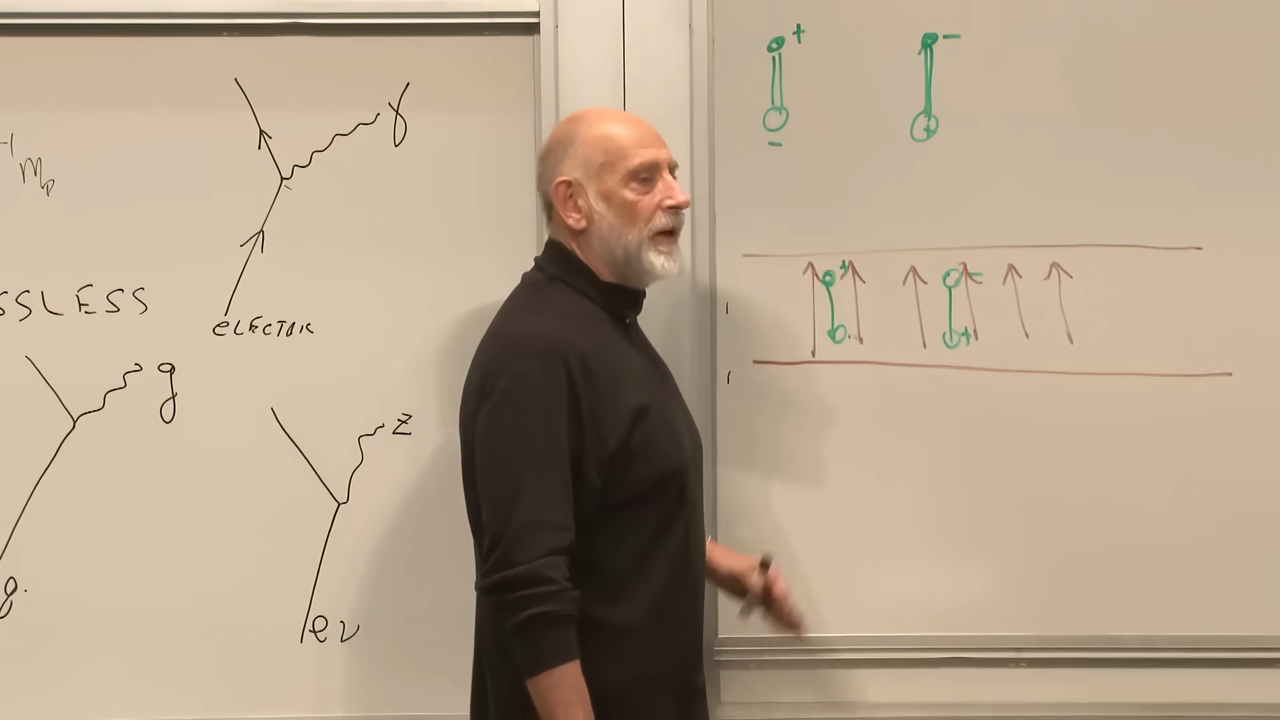
\includegraphics[width=0.95\textwidth]{lecture_144_figure_07.png}
\caption{电容器场中相反的分子取向。该场分裂了它们的能量，却没有引入拖曳力。}
\lectureframe{00:34:35}
\end{figure}

这就排除了两个误导性的类比。希格斯场不是粒子必须费力穿行的糖浆，有质量的粒子也不是被前方堆积的物质拖慢的扫雪车。在空间均匀的场中，根本不必存在净力。其效应是内部能量的移动，而不是摩擦，也不是动量的损失。

同一个例子可以用量子语言重述。经典电场是一个相干态，就目前的目的而言，可以把它描述为光子的凝聚体。分子可以向该背景发射一个光子，或从中吸收一个光子。由于增加或移除单个量子几乎不会改变一个高度占据的相干态，光子线可以终止于凝聚体中。黑板上画的叉号表示这种向背景中的消失，而不是能量守恒的失效。

\begin{figure}[tbp]
\centering
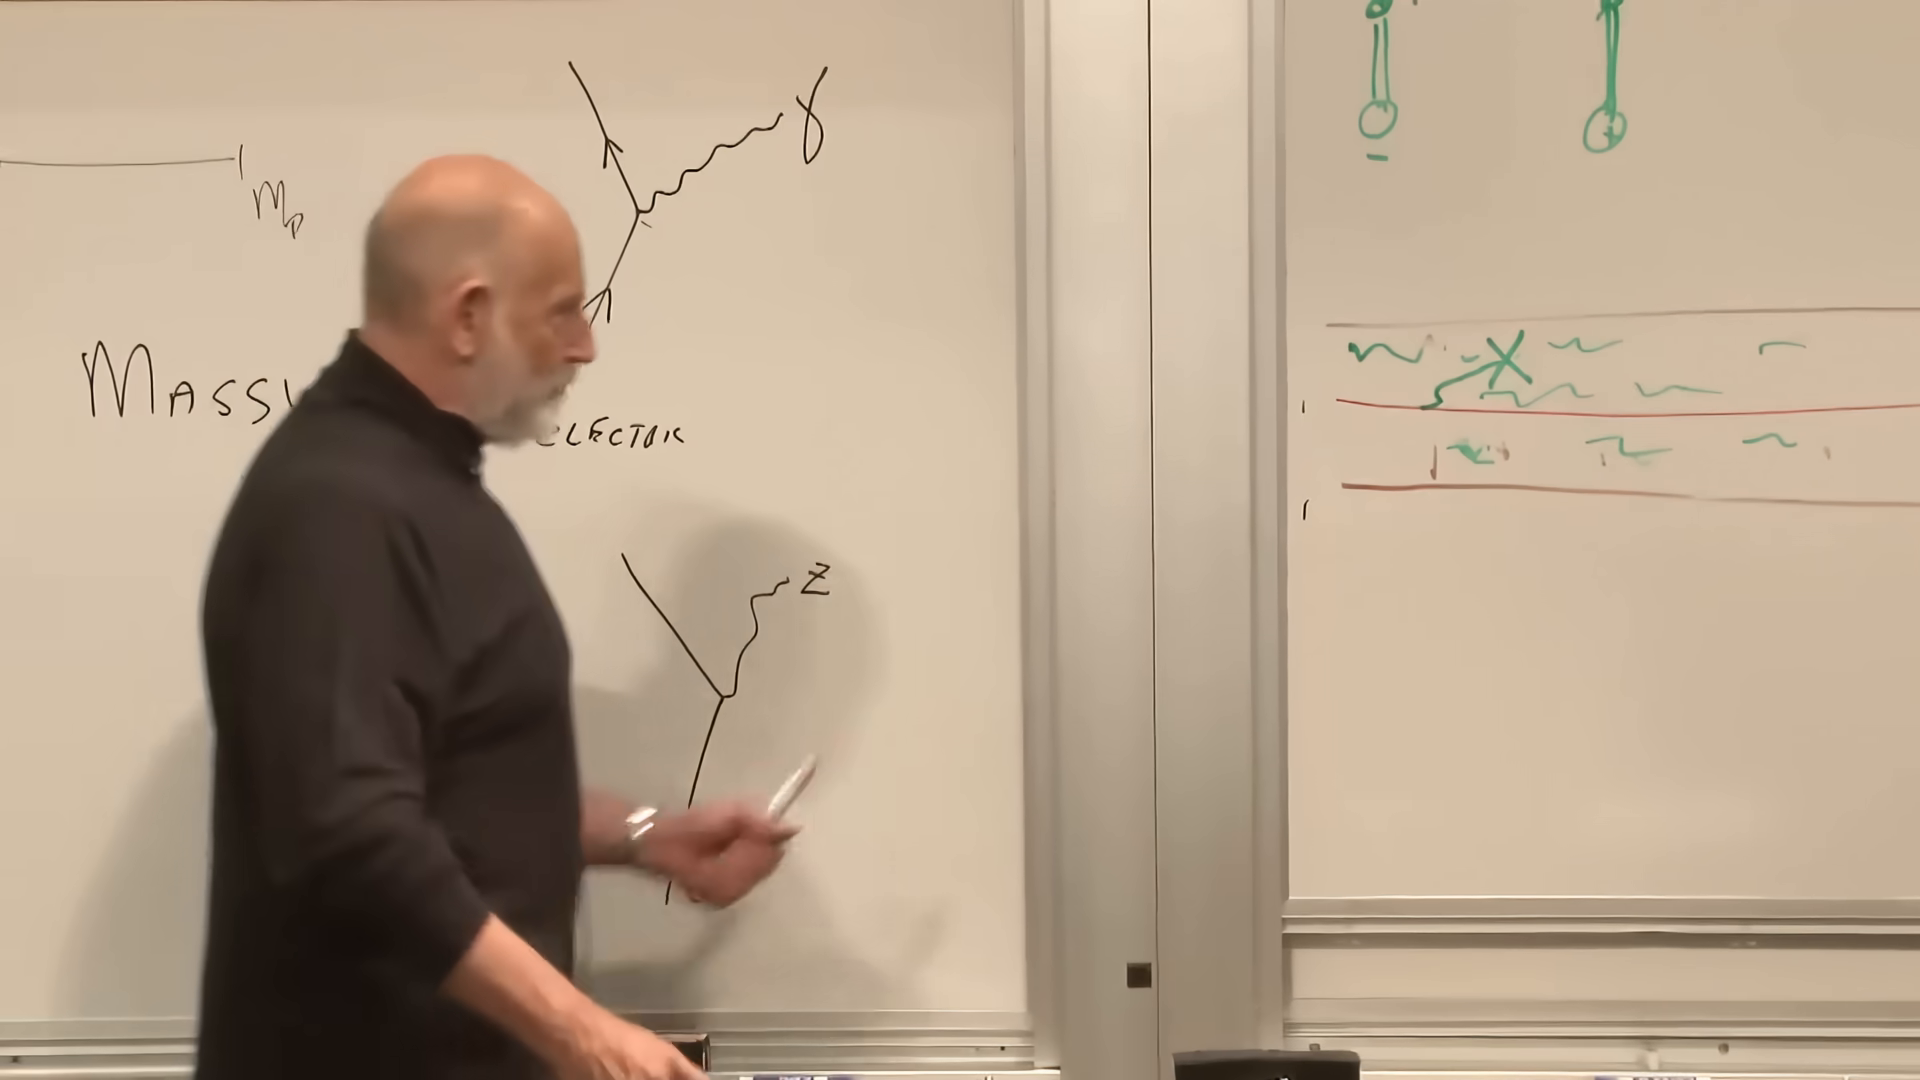
\includegraphics[width=0.95\textwidth]{lecture_144_figure_08.png}
\caption{把电容器场重新画成光子凝聚体。偶极子发射的光子被背景吸收，而背景对多一个量子并不敏感。}
\lectureframe{00:38:45}
\end{figure}

这就是我们需要的模板。如果一个凝聚体能够吸收两个内部状态之间的量子数差，它就能混合这些状态。它们由此产生的振荡可以表现为质量。

\section{为什么希格斯并不解释全部质量}

在应用那个模板之前，必须先消除一个误解。认为每一个有质量的物体都从希格斯场获得其全部质量，这是错误的。

把辐射放入一个完全反射的盒子中。单个光子是无质量的，但封闭的盒子有静止系并储存能量。它的质量增加
\begin{equation}
\Delta M=\frac{E_{\mathrm{radiation}}}{c^{2}}.
\end{equation}
因此，即使组成成分没有静质量，质量也可以由被束缚的动能和场能产生。

质子是重要的真实例子。它包含处于强相互作用状态中的夸克、反夸克和胶子。质子的大部分质量来自它们的动能和束缚能，而不是简单地把少数组成夸克由希格斯机制产生的质量相加。在讲座中强调的估算里，使轻夸克变为无质量只会以大约百分之一的水平改变质子质量。黑洞把这一逻辑要点表现得更加鲜明：黑洞之所以可能有质量，是因为形成它的总能量，而不是因为每一份贡献都先被希格斯场转化为基本粒子的静质量。

希格斯机制有一项更精确的任务。它允许基本费米子和弱规范玻色子获得质量，同时保持底层规范理论的自洽性。

\section{手征性：质量作为左--右混合}

首先关注电子。自旋是一种内禀角动量。对于运动中的粒子，可以比较其自旋方向与动量方向。用讲座中的几何语言来说，右旋电子和左旋电子由这些方向之间的关系来区分。对于无质量粒子，螺旋度和手征性以论证所需的简单方式一致；对于有质量粒子，则必须区分这两个精确概念。

想象反复超越一个有质量的电子。在另一个惯性系中，它的动量反向，而自旋不变，因此与运动方向相关的表观手性可以反转。没有观察者能超越严格无质量的粒子，因为后者总以光速运动。这引出了讲座中的启发式说法：无质量电子保持在一个手征态中，而有质量电子则不断混合左和右。

精确的场论陈述是，狄拉克质量项耦合两个手征场，
\begin{equation}
\mathcal L_m
=
-m_e\bar e e
=
-m_e
\left(
  \bar e_L e_R
  +
  \bar e_R e_L
\right).
\end{equation}
\editorialnote{狄拉克质量项是讲座中``翻转率''图像的标准数学完成。手征混合与质量成正比；字面意义上的时间速率取决于状态和相对论性时间膨胀。}

如果$m_e=0$，则左场和右场独立传播。如果$m_e\ne0$，则方程将它们耦合起来。正是在这个精确意义上，质量衡量左--右混合的强度。

\section{禁止裸质量的守恒定律}

为什么不从一开始就写下混合项？弱相互作用对$e_L$和$e_R$的处理不同。苏斯金德给相关区别起了一个刻意简单的名字：\emph{zilch}。在讲座所用的归一化下，
\begin{equation}
z(e_L)=1,
\qquad
z(e_R)=0.
\end{equation}
两种手征性具有相同的电荷，但弱量子数不同。因此，直接跃迁
\begin{equation}
e_L\longrightarrow e_R
\end{equation}
将无法守恒弱相互作用所携带的量。在未破缺理论中，裸质量项是被禁止的。

\editorialnote{``Zilch''是教学上的简写。在标准模型中，左旋和右旋费米子属于不同的$SU(2)_L\times U(1)_Y$表示，因此直接的狄拉克质量项不是规范不变的。讲座中的赋值$1$和$0$编码了这一差异，而没有复现完整的电弱荷表。}

黑板上把这一阻碍呈现为一条链。右旋电子不能变成左旋电子，除非有别的什么东西带走zilch的差异。同样的障碍也适用于夸克、{\proseunicodefont μ}子和{\proseunicodefont τ}子，一旦提供了缺失的场，其强度就依赖于粒子种类。

\begin{figure}[tbp]
\centering
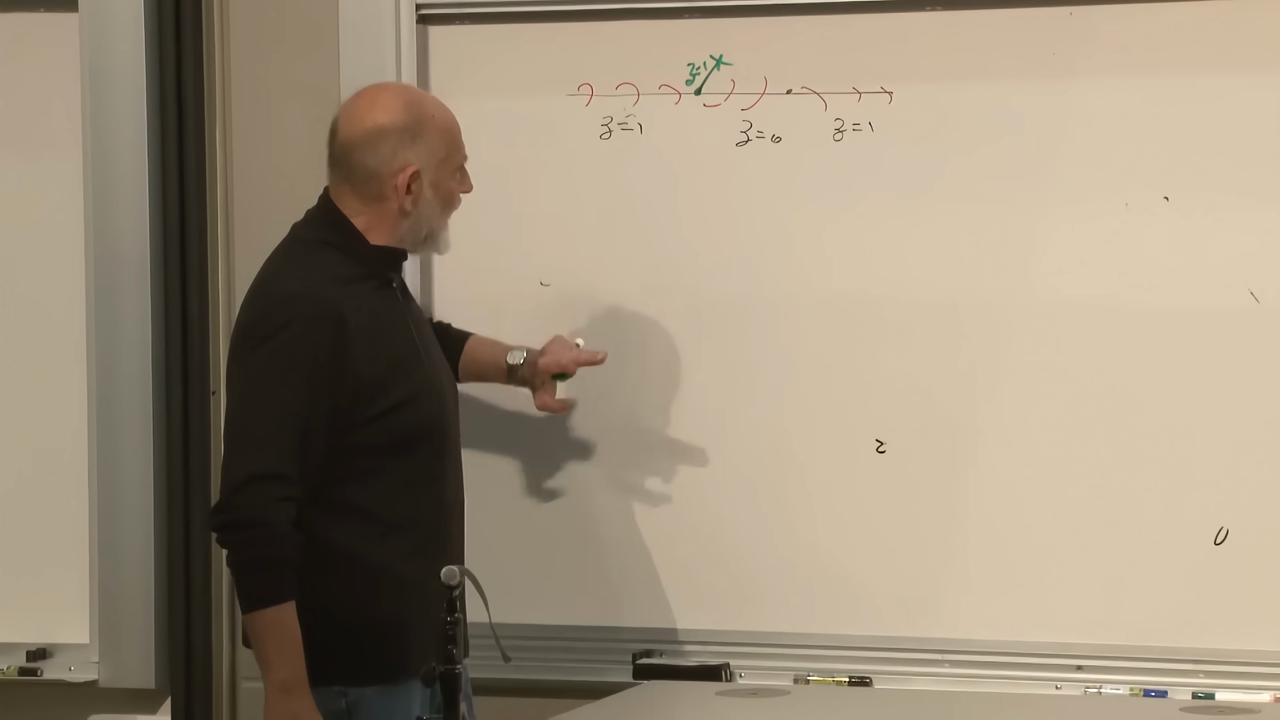
\includegraphics[width=0.95\textwidth]{lecture_144_figure_09.png}
\caption{黑板上的手征序列：在绿色十字处插入一个凝聚体量子，允许zilch标签在右旋和左旋传播之间改变。}
\lectureframe{00:50:15}
\end{figure}

\section{``Ziggs''凝聚体与费米子质量}

引入一个场，其量子恰好携带缺失的弱量子数。为避免过早地与物理希格斯粒子混淆，讲座将其相关的量子称为 \emph{Ziggs}。假设 Ziggs 场具有墨西哥帽势，且其真空是一个凝聚体。那么，一个左手电子可以发射一个 Ziggs 量子并变成右手电子，
\begin{equation}
e_L\longrightarrow e_R+\text{Ziggs},
\end{equation}
或者一个右手电子可以吸收一个并变成左手电子，
\begin{equation}
e_R+\text{Ziggs}\longrightarrow e_L.
\end{equation}
凝聚体吸收或提供量子数差，而不改变其宏观状态。在空的无破缺真空中被禁止的过程，在破缺对称性真空中变为允许。

反复的发射和吸收混合了 $e_L$ 和 $e_R$。因此电子以有质量粒子的形式传播。同样的机制适用于带电轻子和夸克。每个种类与凝聚体有各自的耦合，因此翻转强度以及质量可以因种类而异。

在现代记法中，规范不变相互作用是汤川耦合。在希格斯场获得真空期望值 $v$ 之后，它产生
\begin{equation}
\mathcal L_Y
\supset
-\frac{y_f}{\sqrt{2}}
(v+h)\bar f f,
\end{equation}
因此
\begin{equation}
m_f=\frac{y_fv}{\sqrt{2}},
\qquad
g_{hff}=\frac{y_f}{\sqrt{2}}
=
\frac{m_f}{v}.
\end{equation}
\editorialnote{这些公式提供了讲座的凝聚体耦合论证背后的标准电弱记法。它们也明确说明了为什么同一个耦合同时控制费米子质量和希格斯衰变到该费米子。}

讲座将此描述为手征对称性的自发破缺。这在例子的层面上捕捉了左--右的故事。更精确地说，希格斯期望值将电弱规范对称性破缺到电磁子群，然后汤川相互作用成为费米子质量项。

\section{弱玻色子如何获得质量}

凝聚体也改变了弱规范玻色子。一个 Ziggs 激发可以发射一个 $Z$ 玻色子，反过来 $Z$ 可以变成适当的凝聚体支持的激发并再变回来。因此 $Z$ 在真空中传播，在其中它与希格斯场的角向部分混合。结果是一个有质量的矢量玻色子，具有无质量矢量玻色子所不具备的纵向极化。

\begin{figure}[tbp]
\centering
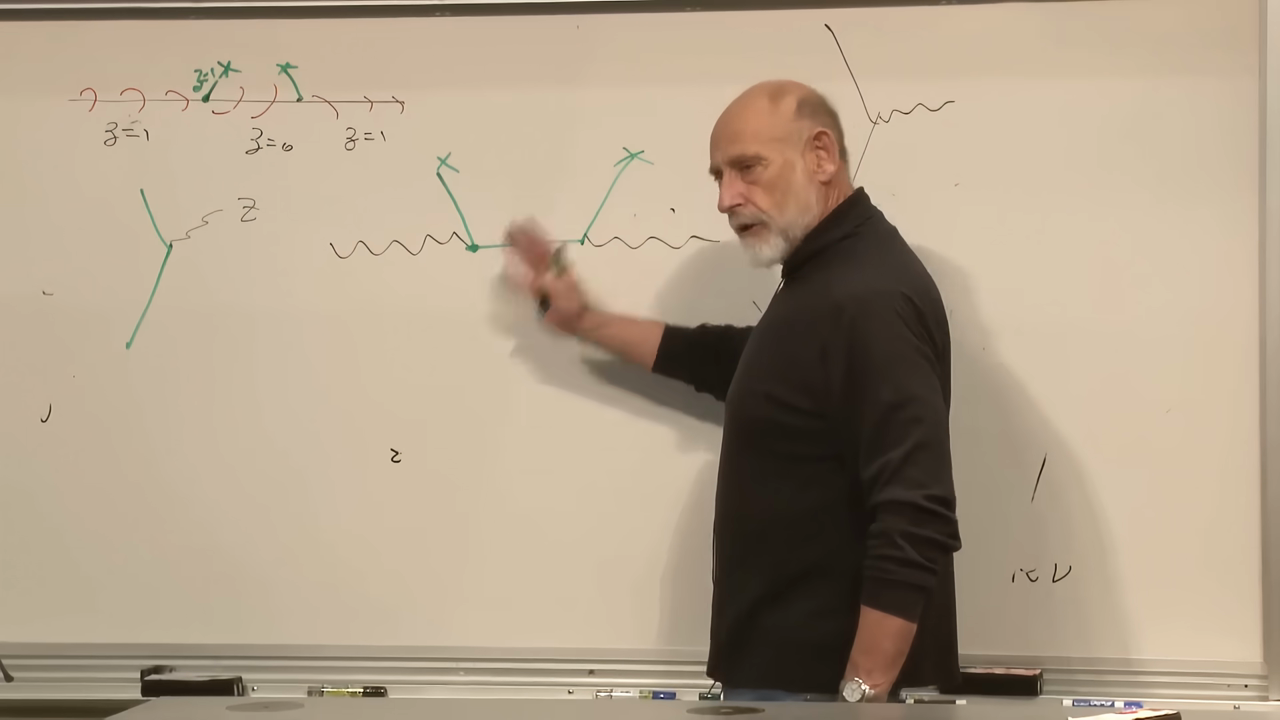
\includegraphics[width=0.95\textwidth]{lecture_144_figure_10.png}
\caption{弱玻色子机制的完整黑板序列：手征链保持在上方，而 $Z$ 在下方与凝聚体支持的部门交换量子数。}
\lectureframe{00:53:40}
\end{figure}

这就是规范玻色子形式的 Brout--Englert--Higgs 现象。在完整的标准模型中，$W$ 玻色子和 $Z$ 都获得质量，而原始中性规范场的一个组合仍然是光子，保持无质量。如果真空反而破缺了普通电磁规范对称性，光子就会获得质量，就像它在超导体内部实际上那样。那时，空的空间将具有完全不同的长程电磁行为。

早在物理希格斯粒子被分离出来之前，弱玻色子就已经为这一机制提供了强有力的证据。它们的质量和相互作用表明电弱对称性以所需的方式破缺。这就是为什么讲座可以在一种宽松的操作意义上说，``Ziggs'' 部门早已为人所知：缺失的实验对象是独立的径向振动。

\editorialnote{讲座中关于 1980 前后在 SLAC 的发现的即兴提及压缩了若干事件。中性弱流在 1973 中被观察到，SLAC 的宇称破坏电子散射在 1970 年代后期被报道，而 $W$ 和 $Z$ 玻色子于 1983 年在 CERN 被直接发现。物理要点是电弱对称性破缺的先期实验确认。}

\section{希格斯玻色子实际上是什么}

回到墨西哥帽。沿谷底的运动会改变角度但不改变半径。该角向部分提供了被有质量弱玻色子吸收的模式。物理希格斯玻色子是另一种运动：沿势阱壁向内和向外的振荡。

将场示意性地写为
\begin{equation}
\Phi(x)
=
\frac{v+h(x)}{\sqrt{2}}
\exp\!\left(
  \frac{i\theta(x)}{v}
\right).
\end{equation}
变量 $\theta$ 描述沿谷底的运动。变量 $h$ 改变半径。在规范理论中，适当的角向自由度成为有质量弱玻色子的纵向分量，而 $h$ 作为传播的标量粒子保留下来：希格斯玻色子。

\begin{figure}[tbp]
\centering
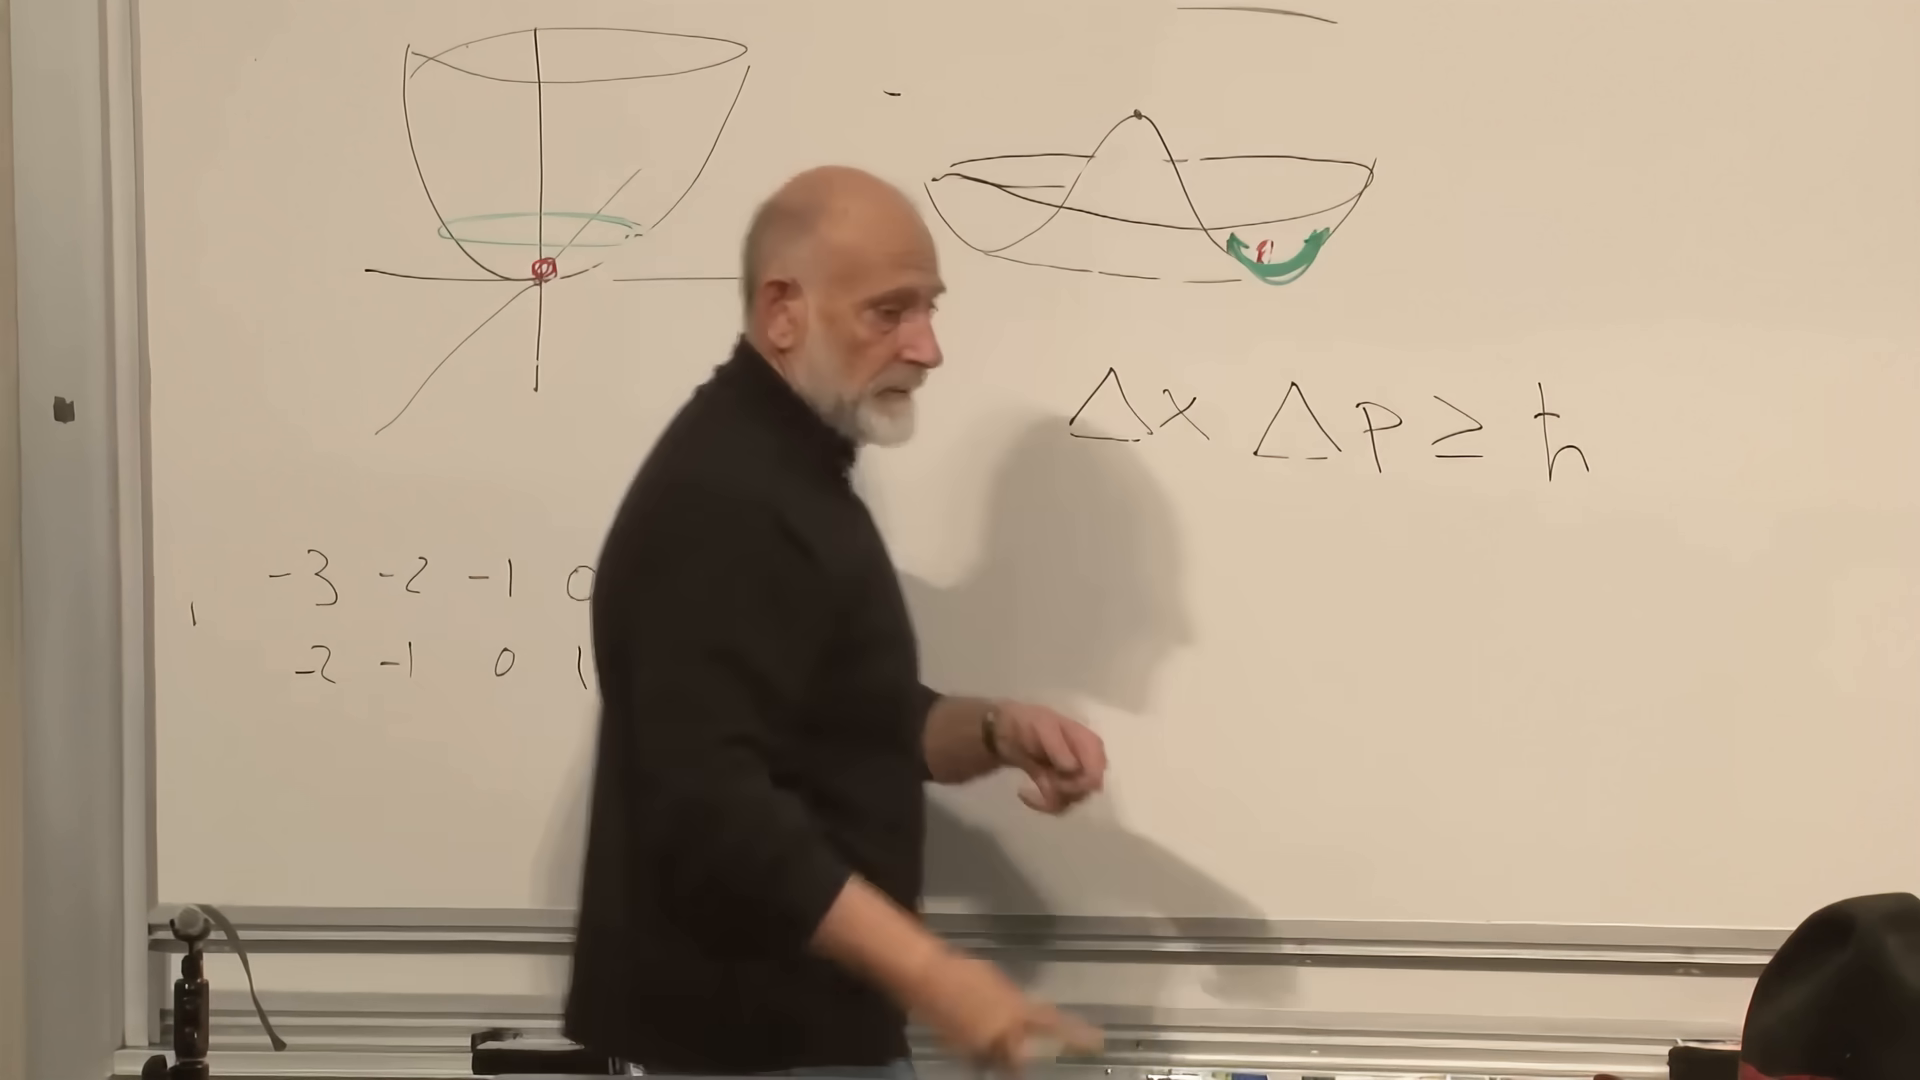
\includegraphics[width=0.95\textwidth]{lecture_144_figure_11.png}
\caption{两个势都重新出现在黑板上，墨西哥帽势阱中标出了径向位移。这种进进出出的振动就是物理希格斯模式。}
\lectureframe{00:56:30}
\end{figure}

存在一种等价的多粒子图像。真空是一种凝聚体，而径向振荡会改变该凝聚体的密度。因此，希格斯玻色子就像该量子介质中的压缩波。只要不由此推断该波必须稳定，这一类比就是有用的。普通声波可以衰减，希格斯激发也可以衰减。

这一区分解释了为什么发现希格斯玻色子是最后缺失的一块拼图，而不是该机制的首个证据。破缺的真空和有质量的弱玻色子早已被间接看到。径向密度波必须作为粒子被产生出来，并通过其衰变产物被识别。

\section{衰变、产生与重费米子优势}

希格斯与费米子的耦合正比于该费米子的质量。它可以衰变为一个费米子-反费米子对，
\begin{equation}
H\longrightarrow f+\bar f,
\end{equation}
而同一张图可以反向解读为产生过程，
\begin{equation}
f+\bar f\longrightarrow H.
\end{equation}
因此电子-正电子湮灭在原理上是可能的。然而从历史上看，早期对撞机首先缺乏足够能量来产生希格斯，而后来的机器则面临更根本的问题：电子汤川耦合极其微小。轻夸克湮灭同样很弱。

\begin{figure}[tbp]
\centering
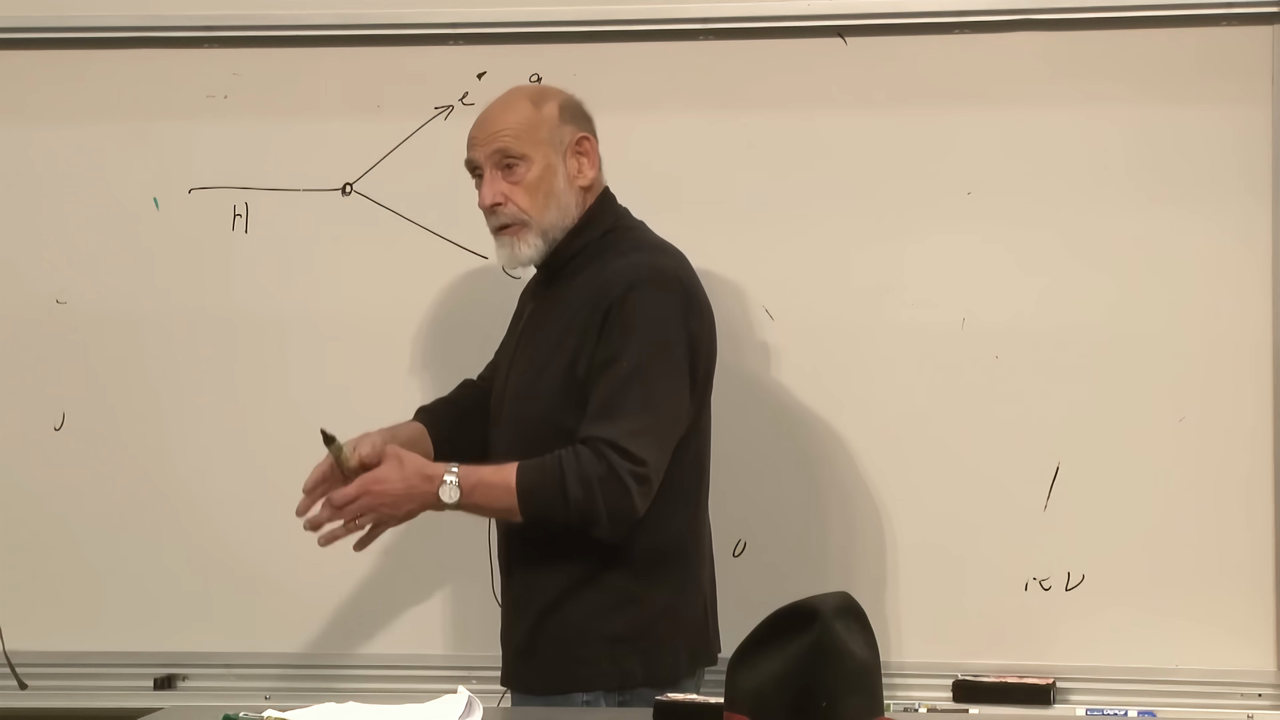
\includegraphics[width=0.95\textwidth]{lecture_144_figure_12.png}
\caption{黑板上画出的希格斯衰变顶点。将箭头反向解读，就得到费米子-反费米子聚合成希格斯。}
\lectureframe{00:59:40}
\end{figure}

费米子越重，其汤川耦合越大。这就使顶夸克格外突出，其质量约为$173\,\mathrm{GeV}$，即大约$180$个质子质量。讲座采用约$170$个质子质量的整数近似。然而，质量接近$125\,\mathrm{GeV}$的希格斯太轻，无法衰变为在壳的$t\bar t$对，
\begin{equation}
m_H<2m_t.
\end{equation}
也无法构建有用的顶夸克束：顶夸克在能够强子化成一种长寿命束流粒子之前就已衰变。

量子力学提供了绕过这两个障碍的办法。两个胶子可以通过一个虚顶夸克圈涨落，并以一个希格斯的形式出现，
\begin{equation}
g+g\longrightarrow H.
\end{equation}
虚顶夸克线不必满足支配真实顶夸克对产生的在壳阈值。质子中充满胶子，因此大型强子对撞机中的高能质子-质子碰撞提供了所需胶子对的强源。

\begin{figure}[tbp]
\centering
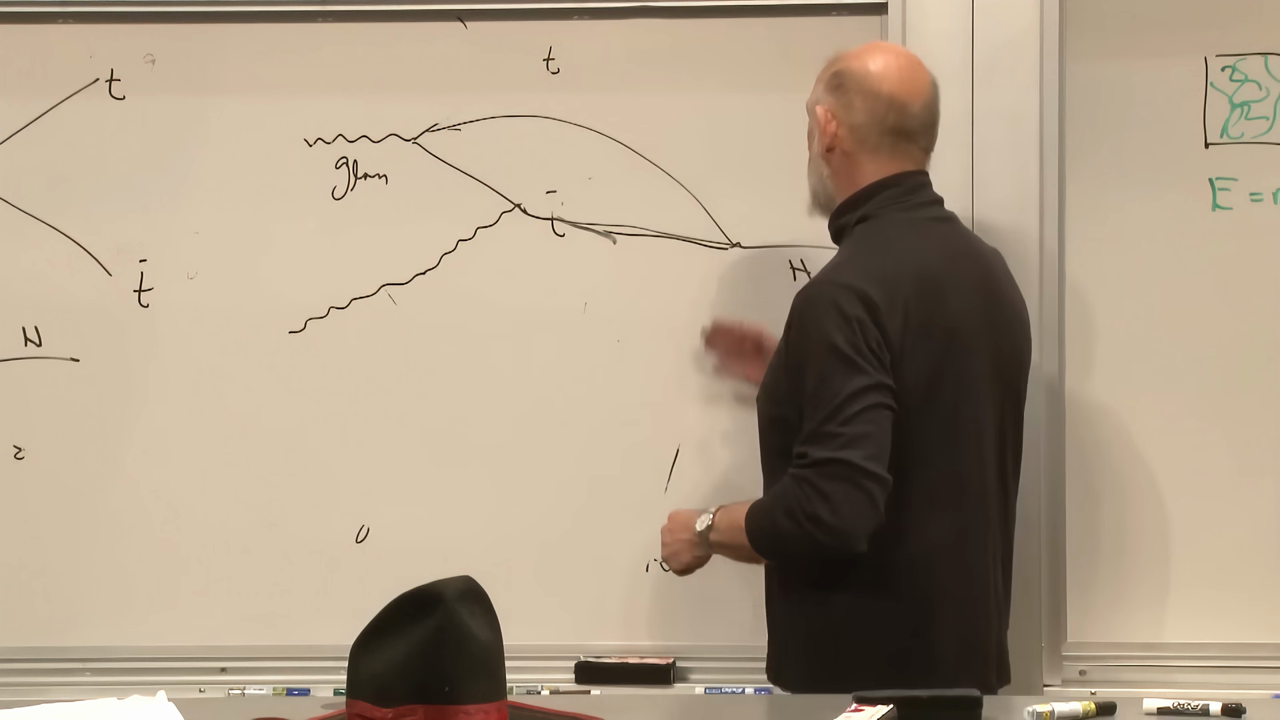
\includegraphics[width=0.95\textwidth]{lecture_144_figure_13.png}
\caption{通过虚顶夸克圈的胶子聚变。取自碰撞质子的两个胶子在圈中相遇并产生希格斯。}
\lectureframe{01:06:35}
\end{figure}

这就是为什么质子对撞机尽管存在质子碎片的复杂性，仍成为决定性的希格斯工厂。质子并不是作为一个基本对象与希格斯耦合；它的胶子组分通过一个由重顶夸克耦合主导的圈产生希格斯。

\section{2012粒子及其双光子检验}

2012中报告的粒子质量接近
\begin{equation}
m_H\simeq125\,\mathrm{GeV}.
\end{equation}
在讲座便于使用的比较中，这大约是$127$个质子质量。它的发现补全了最小标准模型所要求的粒子清单。剩下的问题是，它的定量性质是否恰好就是标准模型的性质。

顶夸克圈的逻辑可以反过来用。希格斯与圈中的虚带电粒子耦合，而该圈可以发射两个光子，
\begin{equation}
H\longrightarrow\gamma+\gamma.
\end{equation}
这种衰变很罕见，但光子在强子对撞机中是异常干净的对象。因此，即使更常见的衰变在实验上更为杂乱，其不变质量分布中的一个窄过剩也可以揭示希格斯。

\begin{figure}[tbp]
\centering
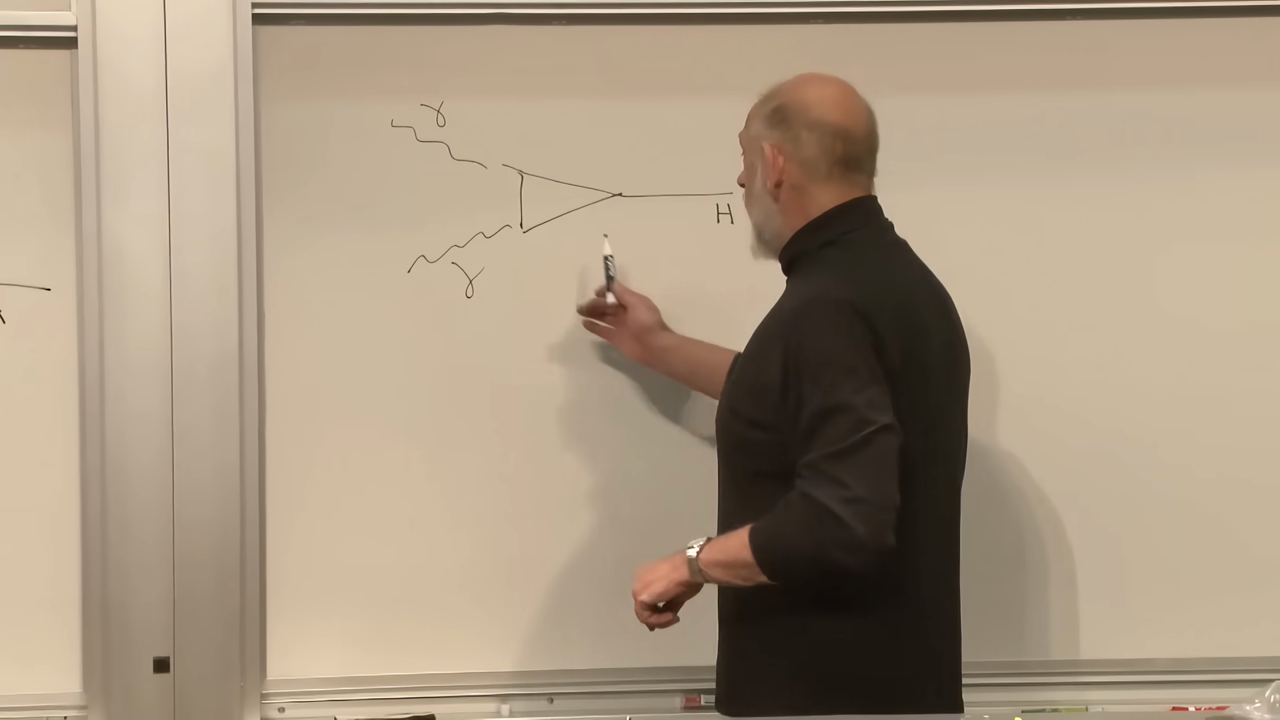
\includegraphics[width=0.95\textwidth]{lecture_144_figure_14.png}
\caption{黑板右侧的双光子三角形，与左侧先前的胶子聚变圈相配。这两个过程从相反方向检验同一圈图层面的逻辑。}
\lectureframe{01:09:00}
\end{figure}

在讲座当时，报告的双光子速率似乎约为最简单标准模型预期的一点五倍，显著性仅约两个标准差。这样的涨落本身并不是证据。然而，如果它持续存在，就可能表明圈中存在一个额外的带电粒子，或许是与超对称或标准模型的另一种扩展相关的粒子。

这一陈述属于2012的历史时刻。它记录的是当时实验学家被告知接下来要关注什么，而不是当前的异常主张。这一发现本身在很大程度上是对一个已由弱玻色子数据支持的框架的确认。科学上更尖锐的检验是衰变速率：这个新标量是否以希格斯机制所预言的、依赖于质量的模式与每个粒子耦合？

\section{听众提问}

\begin{classroomqa}
\audiencequestion{是什么决定了一个费米子比另一个费米子在左右之间振荡得更快，因而具有不同的质量？\lecturetimestamp{01:12:00}}
\lecturerresponse{每一种费米子都有其自身与希格斯凝聚体的耦合。耦合越强，左--右混合就越强，质量也越大。同一个耦合还决定了物理希格斯玻色子衰变到该费米子的强度，这就是为什么较重的费米子通常耦合更强。标准模型将这些汤川耦合参数化，但并未解释它们那引人注目的层级结构。说电子具有小耦合而顶夸克具有大耦合，是一种准确的描述，却还不是更深入的推导。}
\end{classroomqa}

\begin{classroomqa}
\audiencequestion{我们知道真空中希格斯场的量值吗？\lecturetimestamp{01:13:36}}
\lecturerresponse{知道。在本文所用的约定下，真空期望值约为$240\,\mathrm{GeV}$；更精确的标准值约为$246\,\mathrm{GeV}$。它既可以描绘为场从原点的径向位移，也可以描绘为凝聚体的密度。一个物理希格斯量子就是该量值的小幅径向振荡，等价地说是凝聚体的局域密度涨落。}
\end{classroomqa}

\begin{classroomqa}
\audiencequestion{希格斯场的非零真空值是否意味着真空具有能量密度？\lecturetimestamp{01:14:12}}
\lecturerresponse{是的。希格斯势对真空能有贡献，量子场论的许多其他部分也是如此。观测到的净真空能与这些贡献的自然尺度相比极其微小，因此它们必须几乎相互抵消。尚无公认的理论解释这种抵消。这就是宇宙学常数问题，是基础物理学中最深刻的未解问题之一。}
\end{classroomqa}

\section{这一构造所取得的成就}

现在可以不借助黏性以太，从头到尾读懂这一逻辑。量子化的内禀旋转为电荷提供了模型。把碗变成墨西哥帽，使场获得非零真空值。不确定性原理把被精确选定的经典真空变成对单个量子不敏感的凝聚体。于是，凝聚体可以承载左右手费米子之间的弱量子数差，使它们能够混合，从而获得质量。它还提供了纵向模式，使$W$和$Z$能够作为有质量的矢量玻色子传播，而光子保持无质量。

物理希格斯玻色子是在这一重新安排之后仍然存在的径向振荡。它并不是``质量本身，''也不对质子的大部分质量负责。它是对称破缺场的可观测密度波。它的耦合记得由该场产生的质量，这就是为什么重粒子主导其产生和衰变。因此，胶子聚变圈、双光子道，以及听众关于真空能的最后一个问题，并不是彼此无关的奇趣现象。它们是同一个非平凡真空的后果、检验和尚未完成的推论。

\end{document}
